\documentclass[slides]{beamer} %switch "slides" to "handout" for printing out
%\documentclass[handout]{beamer}

%packages
%\usepackage{latexsym}
\usepackage{graphicx}
\usepackage{color}
\usepackage{amsmath}
\usepackage{dsfont}
\usepackage{placeins}
\usepackage{amssymb}
\usepackage{wasysym}
%\usepackage{abstract}
\usepackage{hyperref}
\usepackage{etoolbox}
\usepackage{datetime}
\usepackage{xcolor}
\usepackage{alphalph}
\usepackage[normalem]{ulem}
\settimeformat{ampmtime}

%\usepackage{pstricks,pst-node,pst-tree}

%\usepackage{algpseudocode}
%\usepackage{amsthm}
%\usepackage{hyperref}
%\usepackage{mathrsfs}
%\usepackage{amsfonts}
%\usepackage{bbding}
%\usepackage{listings}
%\usepackage{appendix}
%\usepackage[margin=1in]{geometry}
%\geometry{papersize={8.5in,11in},total={6.5in,9in}}
%\usepackage{cancel}
%\usepackage{algorithmic, algorithm}

\makeatletter
\def\maxwidth{ %
  \ifdim\Gin@nat@width>\linewidth
    \linewidth
  \else
    \Gin@nat@width
  \fi
}
\makeatother

\definecolor{fgcolor}{rgb}{0.345, 0.345, 0.345}
\newcommand{\hlnum}[1]{\textcolor[rgb]{0.686,0.059,0.569}{#1}}%
\newcommand{\hlstr}[1]{\textcolor[rgb]{0.192,0.494,0.8}{#1}}%
\newcommand{\hlcom}[1]{\textcolor[rgb]{0.678,0.584,0.686}{\textit{#1}}}%
\newcommand{\hlopt}[1]{\textcolor[rgb]{0,0,0}{#1}}%
\newcommand{\hlstd}[1]{\textcolor[rgb]{0.345,0.345,0.345}{#1}}%
\newcommand{\hlkwa}[1]{\textcolor[rgb]{0.161,0.373,0.58}{\textbf{#1}}}%
\newcommand{\hlkwb}[1]{\textcolor[rgb]{0.69,0.353,0.396}{#1}}%
\newcommand{\hlkwc}[1]{\textcolor[rgb]{0.333,0.667,0.333}{#1}}%
\newcommand{\hlkwd}[1]{\textcolor[rgb]{0.737,0.353,0.396}{\textbf{#1}}}%

\usepackage{framed}
\makeatletter
\newenvironment{kframe}{%
 \def\at@end@of@kframe{}%
 \ifinner\ifhmode%
  \def\at@end@of@kframe{\end{minipage}}%
  \begin{minipage}{\columnwidth}%
 \fi\fi%
 \def\FrameCommand##1{\hskip\@totalleftmargin \hskip-\fboxsep
 \colorbox{shadecolor}{##1}\hskip-\fboxsep
     % There is no \\@totalrightmargin, so:
     \hskip-\linewidth \hskip-\@totalleftmargin \hskip\columnwidth}%
 \MakeFramed {\advance\hsize-\width
   \@totalleftmargin\z@ \linewidth\hsize
   \@setminipage}}%
 {\par\unskip\endMakeFramed%
 \at@end@of@kframe}
\makeatother

\definecolor{shadecolor}{rgb}{.77, .77, .77}
\definecolor{messagecolor}{rgb}{0, 0, 0}
\definecolor{warningcolor}{rgb}{1, 0, 1}
\definecolor{errorcolor}{rgb}{1, 0, 0}
\newenvironment{knitrout}{}{} % an empty environment to be redefined in TeX

\usepackage{alltt}
\usepackage[T1]{fontenc}

\newcommand{\qu}[1]{``#1''}
\newcounter{probnum}
\setcounter{probnum}{1}

%create definition to allow local margin changes
\def\changemargin#1#2{\list{}{\rightmargin#2\leftmargin#1}\item[]}
\let\endchangemargin=\endlist 

%allow equations to span multiple pages
\allowdisplaybreaks

%define colors and color typesetting conveniences
\definecolor{gray}{rgb}{0.5,0.5,0.5}
\newcommand{\ingray}[1]{\color{gray}#1 \color{black}}
\newcommand{\ingrey}[1]{\ingray{#1}}
\definecolor{black}{rgb}{0,0,0}
\definecolor{white}{rgb}{1,1,1}
\definecolor{blue}{rgb}{0.5,0.5,1}
\newcommand{\inblue}[1]{\color{blue}#1 \color{black}}
\definecolor{green}{rgb}{0.133,0.545,0.133}
\newcommand{\ingreen}[1]{\color{green}#1 \color{black}}
\definecolor{yellow}{rgb}{1,1,0}
\newcommand{\inyellow}[1]{\color{yellow}#1 \color{black}}
\definecolor{orange}{rgb}{0.9,0.649,0}
\newcommand{\inorange}[1]{\color{orange}#1 \color{black}}
\definecolor{red}{rgb}{1,0.133,0.133}
\newcommand{\inred}[1]{\color{red}#1 \color{black}}
\definecolor{purple}{rgb}{0.58,0,0.827}
\newcommand{\inpurple}[1]{\color{purple}#1 \color{black}}
\definecolor{backgcode}{rgb}{0.97,0.97,0.8}
\definecolor{Brown}{cmyk}{0,0.81,1,0.60}
\definecolor{OliveGreen}{cmyk}{0.64,0,0.95,0.40}
\definecolor{CadetBlue}{cmyk}{0.62,0.57,0.23,0}

%define new math operators
\DeclareMathOperator*{\argmax}{arg\,max~}
\DeclareMathOperator*{\argmin}{arg\,min~}
\DeclareMathOperator*{\argsup}{arg\,sup~}
\DeclareMathOperator*{\arginf}{arg\,inf~}
\DeclareMathOperator*{\convolution}{\text{\Huge{$\ast$}}}
\newcommand{\infconv}[2]{\convolution^\infty_{#1 = 1} #2}
%true functions

%%%% GENERAL SHORTCUTS

%shortcuts for pure typesetting conveniences
\newcommand{\bv}[1]{\boldsymbol{#1}}

%shortcuts for compound constants
\newcommand{\BetaDistrConst}{\dfrac{\Gamma(\alpha + \beta)}{\Gamma(\alpha)\Gamma(\beta)}}
\newcommand{\NormDistrConst}{\dfrac{1}{\sqrt{2\pi\sigma^2}}}

%shortcuts for conventional symbols
\newcommand{\tsq}{\tau^2}
\newcommand{\tsqh}{\hat{\tau}^2}
\newcommand{\sigsq}{\sigma^2}
\newcommand{\sigsqsq}{\parens{\sigma^2}^2}
\newcommand{\sigsqovern}{\dfrac{\sigsq}{n}}
\newcommand{\tausq}{\tau^2}
\newcommand{\tausqalpha}{\tau^2_\alpha}
\newcommand{\tausqbeta}{\tau^2_\beta}
\newcommand{\tausqsigma}{\tau^2_\sigma}
\newcommand{\betasq}{\beta^2}
\newcommand{\sigsqvec}{\bv{\sigma}^2}
\newcommand{\sigsqhat}{\hat{\sigma}^2}
\newcommand{\sigsqhatmlebayes}{\sigsqhat_{\text{Bayes, MLE}}}
\newcommand{\sigsqhatmle}[1]{\sigsqhat_{#1, \text{MLE}}}
\newcommand{\bSigma}{\bv{\Sigma}}
\newcommand{\bSigmainv}{\bSigma^{-1}}
\newcommand{\thetavec}{\bv{\theta}}
\newcommand{\thetahat}{\hat{\theta}}
\newcommand{\thetahatmle}{\hat{\theta}_{\mathrm{MLE}}}
\newcommand{\thetavechatmle}{\hat{\thetavec}_{\mathrm{MLE}}}
\newcommand{\muhat}{\hat{\mu}}
\newcommand{\musq}{\mu^2}
\newcommand{\muvec}{\bv{\mu}}
\newcommand{\muhatmle}{\muhat_{\text{MLE}}}
\newcommand{\lambdahat}{\hat{\lambda}}
\newcommand{\lambdahatmle}{\lambdahat_{\text{MLE}}}
\newcommand{\etavec}{\bv{\eta}}
\newcommand{\alphavec}{\bv{\alpha}}
\newcommand{\minimaxdec}{\delta^*_{\mathrm{mm}}}
\newcommand{\ybar}{\bar{y}}
\newcommand{\xbar}{\bar{x}}
\newcommand{\Xbar}{\bar{X}}
\newcommand{\phat}{\hat{p}}
\newcommand{\Phat}{\hat{P}}
\newcommand{\Zbar}{\bar{Z}}
\newcommand{\iid}{~{\buildrel iid \over \sim}~}
\newcommand{\inddist}{~{\buildrel ind \over \sim}~}
\newcommand{\approxdist}{~{\buildrel approx \over \sim}~}
\newcommand{\equalsindist}{~{\buildrel d \over =}~}
\newcommand{\lik}[1]{\mathcal{L}\parens{#1}}
\newcommand{\loglik}[1]{\ell\parens{#1}}
\newcommand{\thetahatkminone}{\thetahat^{(k-1)}}
\newcommand{\thetahatkplusone}{\thetahat^{(k+1)}}
\newcommand{\thetahatk}{\thetahat^{(k)}}
\newcommand{\half}{\frac{1}{2}}
\newcommand{\third}{\frac{1}{3}}
\newcommand{\twothirds}{\frac{2}{3}}
\newcommand{\fourth}{\frac{1}{4}}
\newcommand{\fifth}{\frac{1}{5}}
\newcommand{\sixth}{\frac{1}{6}}

%shortcuts for vector and matrix notation
\newcommand{\A}{\bv{A}}
\newcommand{\At}{\A^T}
\newcommand{\Ainv}{\inverse{\A}}
\newcommand{\B}{\bv{B}}
\newcommand{\K}{\bv{K}}
\newcommand{\Kt}{\K^T}
\newcommand{\Kinv}{\inverse{K}}
\newcommand{\Kinvt}{(\Kinv)^T}
\newcommand{\M}{\bv{M}}
\newcommand{\Bt}{\B^T}
\newcommand{\Q}{\bv{Q}}
\newcommand{\Qt}{\Q^T}
\newcommand{\R}{\bv{R}}
\newcommand{\Rt}{\R^T}
\newcommand{\Z}{\bv{Z}}
\newcommand{\X}{\bv{X}}
\newcommand{\Xsub}{\X_{\text{(sub)}}}
\newcommand{\Xsubadj}{\X_{\text{(sub,adj)}}}
\newcommand{\I}{\bv{I}}
\newcommand{\Y}{\bv{Y}}
\newcommand{\sigsqI}{\sigsq\I}
\renewcommand{\P}{\bv{P}}
\newcommand{\Psub}{\P_{\text{(sub)}}}
\newcommand{\Pt}{\P^T}
\newcommand{\Pii}{P_{ii}}
\newcommand{\Pij}{P_{ij}}
\newcommand{\IminP}{(\I-\P)}
\newcommand{\Xt}{\bv{X}^T}
\newcommand{\XtX}{\Xt\X}
\newcommand{\XtXinv}{\parens{\Xt\X}^{-1}}
\newcommand{\XtXinvXt}{\XtXinv\Xt}
\newcommand{\XXtXinvXt}{\X\XtXinvXt}
\newcommand{\x}{\bv{x}}
\newcommand{\onevec}{\bv{1}}
\newcommand{\oneton}{1, \ldots, n}
\newcommand{\yoneton}{y_1, \ldots, y_n}
\newcommand{\yonetonorder}{y_{(1)}, \ldots, y_{(n)}}
\newcommand{\Yoneton}{Y_1, \ldots, Y_n}
\newcommand{\iinoneton}{i \in \braces{\oneton}}
\newcommand{\onetom}{1, \ldots, m}
\newcommand{\jinonetom}{j \in \braces{\onetom}}
\newcommand{\xoneton}{x_1, \ldots, x_n}
\newcommand{\Xoneton}{X_1, \ldots, X_n}
\newcommand{\xt}{\x^T}
\newcommand{\y}{\bv{y}}
\newcommand{\yt}{\y^T}
\renewcommand{\c}{\bv{c}}
\newcommand{\ct}{\c^T}
\newcommand{\tstar}{\bv{t}^*}
\renewcommand{\u}{\bv{u}}
\renewcommand{\v}{\bv{v}}
\renewcommand{\a}{\bv{a}}
\newcommand{\s}{\bv{s}}
\newcommand{\yadj}{\y_{\text{(adj)}}}
\newcommand{\xjadj}{\x_{j\text{(adj)}}}
\newcommand{\xjadjM}{\x_{j \perp M}}
\newcommand{\yhat}{\hat{y}}
\newcommand{\fhat}{\hat{f}}
\newcommand{\betahat}{\hat{\beta}}
\newcommand{\yhatsub}{\yhat_{\text{(sub)}}}
\newcommand{\yhatstar}{\yhat^*}
\newcommand{\yhatstarnew}{\yhatstar_{\text{new}}}
\newcommand{\z}{\bv{z}}
\newcommand{\zt}{\z^T}
\newcommand{\bb}{\bv{b}}
\newcommand{\bbt}{\bb^T}
\newcommand{\bbeta}{\bv{\beta}}
\newcommand{\beps}{\bv{\epsilon}}
\newcommand{\bepst}{\beps^T}
\newcommand{\e}{\bv{e}}
\newcommand{\Mofy}{\M(\y)}
\newcommand{\KofAlpha}{K(\alpha)}
\newcommand{\ellset}{\mathcal{L}}
\newcommand{\oneminalph}{1-\alpha}
\newcommand{\SSE}{\text{SSE}}
\newcommand{\SSEsub}{\text{SSE}_{\text{(sub)}}}
\newcommand{\MSE}{\text{MSE}}
\newcommand{\RMSE}{\text{RMSE}}
\newcommand{\SSR}{\text{SSR}}
\newcommand{\SST}{\text{SST}}
\newcommand{\JSest}{\delta_{\text{JS}}(\x)}
\newcommand{\Bayesest}{\delta_{\text{Bayes}}(\x)}
\newcommand{\EmpBayesest}{\delta_{\text{EmpBayes}}(\x)}
\newcommand{\BLUPest}{\delta_{\text{BLUP}}}
\newcommand{\MLEest}[1]{\hat{#1}_{\text{MLE}}}

%shortcuts for Linear Algebra stuff (i.e. vectors and matrices)
\newcommand{\twovec}[2]{\bracks{\begin{array}{c} #1 \\ #2 \end{array}}}
\newcommand{\threevec}[3]{\bracks{\begin{array}{c} #1 \\ #2 \\ #3 \end{array}}}
\newcommand{\fivevec}[5]{\bracks{\begin{array}{c} #1 \\ #2 \\ #3 \\ #4 \\ #5 \end{array}}}
\newcommand{\twobytwomat}[4]{\bracks{\begin{array}{cc} #1 & #2 \\ #3 & #4 \end{array}}}
\newcommand{\threebytwomat}[6]{\bracks{\begin{array}{cc} #1 & #2 \\ #3 & #4 \\ #5 & #6 \end{array}}}

%shortcuts for conventional compound symbols
\newcommand{\thetainthetas}{\theta \in \Theta}
\newcommand{\reals}{\mathbb{R}}
\newcommand{\complexes}{\mathbb{C}}
\newcommand{\rationals}{\mathbb{Q}}
\newcommand{\integers}{\mathbb{Z}}
\newcommand{\naturals}{\mathbb{N}}
\newcommand{\forallninN}{~~\forall n \in \naturals}
\newcommand{\forallxinN}[1]{~~\forall #1 \in \reals}
\newcommand{\matrixdims}[2]{\in \reals^{\,#1 \times #2}}
\newcommand{\inRn}[1]{\in \reals^{\,#1}}
\newcommand{\mathimplies}{\quad\Rightarrow\quad}
\newcommand{\mathlogicequiv}{\quad\Leftrightarrow\quad}
\newcommand{\eqncomment}[1]{\quad \text{(#1)}}
\newcommand{\limitn}{\lim_{n \rightarrow \infty}}
\newcommand{\limitN}{\lim_{N \rightarrow \infty}}
\newcommand{\limitd}{\lim_{d \rightarrow \infty}}
\newcommand{\limitt}{\lim_{t \rightarrow \infty}}
\newcommand{\limitsupn}{\limsup_{n \rightarrow \infty}~}
\newcommand{\limitinfn}{\liminf_{n \rightarrow \infty}~}
\newcommand{\limitk}{\lim_{k \rightarrow \infty}}
\newcommand{\limsupn}{\limsup_{n \rightarrow \infty}}
\newcommand{\limsupk}{\limsup_{k \rightarrow \infty}}
\newcommand{\floor}[1]{\left\lfloor #1 \right\rfloor}
\newcommand{\ceil}[1]{\left\lceil #1 \right\rceil}

%shortcuts for environments
\newcommand{\beqn}{\vspace{-0.25cm}\begin{eqnarray*}}
\newcommand{\eeqn}{\end{eqnarray*}}
\newcommand{\bneqn}{\vspace{-0.25cm}\begin{eqnarray}}
\newcommand{\eneqn}{\end{eqnarray}}

%shortcuts for mini environments
\newcommand{\parens}[1]{\left(#1\right)}
\newcommand{\squared}[1]{\parens{#1}^2}
\newcommand{\tothepow}[2]{\parens{#1}^{#2}}
\newcommand{\prob}[1]{\mathbb{P}\parens{#1}}
\newcommand{\cprob}[2]{\prob{#1~|~#2}}
\newcommand{\littleo}[1]{o\parens{#1}}
\newcommand{\bigo}[1]{O\parens{#1}}
\newcommand{\Lp}[1]{\mathbb{L}^{#1}}
\renewcommand{\arcsin}[1]{\text{arcsin}\parens{#1}}
\newcommand{\prodonen}[2]{\bracks{\prod_{#1=1}^n #2}}
\newcommand{\mysum}[4]{\sum_{#1=#2}^{#3} #4}
\newcommand{\sumonen}[2]{\sum_{#1=1}^n #2}
\newcommand{\sumionen}[1]{\sumonen{i}{#1}}
\newcommand{\infsum}[2]{\sum_{#1=1}^\infty #2}
\newcommand{\infprod}[2]{\prod_{#1=1}^\infty #2}
\newcommand{\infunion}[2]{\bigcup_{#1=1}^\infty #2}
\newcommand{\infinter}[2]{\bigcap_{#1=1}^\infty #2}
\newcommand{\infintegral}[2]{\int^\infty_{-\infty} #2 ~\text{d}#1}
\newcommand{\supthetas}[1]{\sup_{\thetainthetas}\braces{#1}}
\newcommand{\bracks}[1]{\left[#1\right]}
\newcommand{\braces}[1]{\left\{#1\right\}}
\newcommand{\angbraces}[1]{\left<#1\right>}
\newcommand{\set}[1]{\left\{#1\right\}}
\newcommand{\abss}[1]{\left|#1\right|}
\newcommand{\norm}[1]{\left|\left|#1\right|\right|}
\newcommand{\normsq}[1]{\norm{#1}^2}
\newcommand{\inverse}[1]{\parens{#1}^{-1}}
\newcommand{\rowof}[2]{\parens{#1}_{#2\cdot}}

%shortcuts for functionals
\newcommand{\realcomp}[1]{\text{Re}\bracks{#1}}
\newcommand{\imagcomp}[1]{\text{Im}\bracks{#1}}
\newcommand{\range}[1]{\text{range}\bracks{#1}}
\newcommand{\colsp}[1]{\text{colsp}\bracks{#1}}
\newcommand{\rowsp}[1]{\text{rowsp}\bracks{#1}}
\newcommand{\tr}[1]{\text{tr}\bracks{#1}}
\newcommand{\rank}[1]{\text{rank}\bracks{#1}}
\newcommand{\proj}[2]{\text{Proj}_{#1}\bracks{#2}}
\newcommand{\projcolspX}[1]{\text{Proj}_{\colsp{\X}}\bracks{#1}}
\newcommand{\median}[1]{\text{median}\bracks{#1}}
\newcommand{\mean}[1]{\text{mean}\bracks{#1}}
\newcommand{\dime}[1]{\text{dim}\bracks{#1}}
\renewcommand{\det}[1]{\text{det}\bracks{#1}}
\newcommand{\expe}[1]{\mathbb{E}\bracks{#1}}
\newcommand{\cexpe}[2]{\expe{#1~|~#2}}
\newcommand{\expeabs}[1]{\expe{\abss{#1}}}
\newcommand{\expesub}[2]{\mathbb{E}_{#1}\bracks{#2}}
\newcommand{\indic}[1]{\mathds{1}_{#1}}
\newcommand{\var}[1]{\mathbb{V}\text{ar}\bracks{#1}}
\newcommand{\cov}[2]{\mathbb{C}\text{ov}\bracks{#1, #2}}
\newcommand{\corr}[2]{\text{Corr}\bracks{#1, #2}}
\newcommand{\se}[1]{\mathbb{S}\text{E}\bracks{#1}}
\newcommand{\seest}[1]{\hat{\text{SE}}\bracks{#1}}
\newcommand{\bias}[1]{\text{Bias}\bracks{#1}}
\newcommand{\derivop}[2]{\dfrac{\text{d}}{\text{d} #1}\bracks{#2}}
\newcommand{\partialop}[2]{\dfrac{\partial}{\partial #1}\bracks{#2}}
\newcommand{\secpartialop}[2]{\dfrac{\partial^2}{\partial #1^2}\bracks{#2}}
\newcommand{\mixpartialop}[3]{\dfrac{\partial^2}{\partial #1 \partial #2}\bracks{#3}}

%shortcuts for functions
\renewcommand{\exp}[1]{\mathrm{exp}\parens{#1}}
\renewcommand{\cos}[1]{\text{cos}\parens{#1}}
\renewcommand{\sin}[1]{\text{sin}\parens{#1}}
\newcommand{\sign}[1]{\text{sign}\parens{#1}}
\newcommand{\are}[1]{\mathrm{ARE}\parens{#1}}
\newcommand{\natlog}[1]{\ln\parens{#1}}
\newcommand{\oneover}[1]{\frac{1}{#1}}
\newcommand{\overtwo}[1]{\frac{#1}{2}}
\newcommand{\overn}[1]{\frac{#1}{n}}
\newcommand{\oneoversqrt}[1]{\oneover{\sqrt{#1}}}
\newcommand{\sqd}[1]{\parens{#1}^2}
\newcommand{\loss}[1]{\ell\parens{\theta, #1}}
\newcommand{\losstwo}[2]{\ell\parens{#1, #2}}
\newcommand{\cf}{\phi(t)}

%English language specific shortcuts
\newcommand{\ie}{\textit{i.e.} }
\newcommand{\AKA}{\textit{AKA} }
\renewcommand{\iff}{\textit{iff}}
\newcommand{\eg}{\textit{e.g.} }
\newcommand{\st}{\textit{s.t.} }
\newcommand{\wrt}{\textit{w.r.t.} }
\newcommand{\mathst}{~~\text{\st}~~}
\newcommand{\mathand}{~~\text{and}~~}
\newcommand{\ala}{\textit{a la} }
\newcommand{\ppp}{posterior predictive p-value}
\newcommand{\dd}{dataset-to-dataset}

%shortcuts for distribution titles
\newcommand{\logistic}[2]{\mathrm{Logistic}\parens{#1,\,#2}}
\newcommand{\bernoulli}[1]{\mathrm{Bernoulli}\parens{#1}}
\newcommand{\betanot}[2]{\mathrm{Beta}\parens{#1,\,#2}}
\newcommand{\stdbetanot}{\betanot{\alpha}{\beta}}
\newcommand{\multnormnot}[3]{\mathcal{N}_{#1}\parens{#2,\,#3}}
\newcommand{\normnot}[2]{\mathcal{N}\parens{#1,\,#2}}
\newcommand{\classicnormnot}{\normnot{\mu}{\sigsq}}
\newcommand{\stdnormnot}{\normnot{0}{1}}
\newcommand{\uniformdiscrete}[1]{\mathrm{Uniform}\parens{\braces{#1}}}
\newcommand{\uniform}[2]{\mathrm{U}\parens{#1,\,#2}}
\newcommand{\stduniform}{\uniform{0}{1}}
\newcommand{\geometric}[1]{\mathrm{Geometric}\parens{#1}}
\newcommand{\hypergeometric}[3]{\mathrm{Hypergeometric}\parens{#1,\,#2,\,#3}}
\newcommand{\exponential}[1]{\mathrm{Exp}\parens{#1}}
\newcommand{\gammadist}[2]{\mathrm{Gamma}\parens{#1, #2}}
\newcommand{\poisson}[1]{\mathrm{Poisson}\parens{#1}}
\newcommand{\binomial}[2]{\mathrm{Binomial}\parens{#1,\,#2}}
\newcommand{\negbin}[2]{\mathrm{NegBin}\parens{#1,\,#2}}
\newcommand{\rayleigh}[1]{\mathrm{Rayleigh}\parens{#1}}
\newcommand{\multinomial}[2]{\mathrm{Multinomial}\parens{#1,\,#2}}
\newcommand{\gammanot}[2]{\mathrm{Gamma}\parens{#1,\,#2}}
\newcommand{\cauchynot}[2]{\text{Cauchy}\parens{#1,\,#2}}
\newcommand{\invchisqnot}[1]{\text{Inv}\chisq{#1}}
\newcommand{\invscaledchisqnot}[2]{\text{ScaledInv}\ncchisq{#1}{#2}}
\newcommand{\invgammanot}[2]{\text{InvGamma}\parens{#1,\,#2}}
\newcommand{\chisq}[1]{\chi^2_{#1}}
\newcommand{\ncchisq}[2]{\chi^2_{#1}\parens{#2}}
\newcommand{\ncF}[3]{F_{#1,#2}\parens{#3}}

%shortcuts for PDF's of common distributions
\newcommand{\logisticpdf}[3]{\oneover{#3}\dfrac{\exp{-\dfrac{#1 - #2}{#3}}}{\parens{1+\exp{-\dfrac{#1 - #2}{#3}}}^2}}
\newcommand{\betapdf}[3]{\dfrac{\Gamma(#2 + #3)}{\Gamma(#2)\Gamma(#3)}#1^{#2-1} (1-#1)^{#3-1}}
\newcommand{\normpdf}[3]{\frac{1}{\sqrt{2\pi#3}}\exp{-\frac{1}{2#3}(#1 - #2)^2}}
\newcommand{\normpdfvarone}[2]{\dfrac{1}{\sqrt{2\pi}}e^{-\half(#1 - #2)^2}}
\newcommand{\chisqpdf}[2]{\dfrac{1}{2^{#2/2}\Gamma(#2/2)}\; {#1}^{#2/2-1} e^{-#1/2}}
\newcommand{\invchisqpdf}[2]{\dfrac{2^{-\overtwo{#1}}}{\Gamma(#2/2)}\,{#1}^{-\overtwo{#2}-1}  e^{-\oneover{2 #1}}}
\newcommand{\exponentialpdf}[2]{#2\exp{-#2#1}}
\newcommand{\poissonpdf}[2]{\dfrac{e^{-#1} #1^{#2}}{#2!}}
\newcommand{\binomialpdf}[3]{\binom{#2}{#1}#3^{#1}(1-#3)^{#2-#1}}
\newcommand{\rayleighpdf}[2]{\dfrac{#1}{#2^2}\exp{-\dfrac{#1^2}{2 #2^2}}}
\newcommand{\gammapdf}[3]{\dfrac{#3^#2}{\Gamma\parens{#2}}#1^{#2-1}\exp{-#3 #1}}
\newcommand{\cauchypdf}[3]{\oneover{\pi} \dfrac{#3}{\parens{#1-#2}^2 + #3^2}}
\newcommand{\Gammaf}[1]{\Gamma\parens{#1}}

%shortcuts for miscellaneous typesetting conveniences
\newcommand{\notesref}[1]{\marginpar{\color{gray}\tt #1\color{black}}}

%%%% DOMAIN-SPECIFIC SHORTCUTS

%Real analysis related shortcuts
\newcommand{\zeroonecl}{\bracks{0,1}}
\newcommand{\forallepsgrzero}{\forall \epsilon > 0~~}
\newcommand{\lessthaneps}{< \epsilon}
\newcommand{\fraccomp}[1]{\text{frac}\bracks{#1}}

%Bayesian related shortcuts
\newcommand{\yrep}{y^{\text{rep}}}
\newcommand{\yrepisq}{(\yrep_i)^2}
\newcommand{\yrepvec}{\bv{y}^{\text{rep}}}


%Probability shortcuts
\newcommand{\SigField}{\mathcal{F}}
\newcommand{\ProbMap}{\mathcal{P}}
\newcommand{\probtrinity}{\parens{\Omega, \SigField, \ProbMap}}
\newcommand{\convp}{~{\buildrel p \over \rightarrow}~}
\newcommand{\convLp}[1]{~{\buildrel \Lp{#1} \over \rightarrow}~}
\newcommand{\nconvp}{~{\buildrel p \over \nrightarrow}~}
\newcommand{\convae}{~{\buildrel a.e. \over \longrightarrow}~}
\newcommand{\convau}{~{\buildrel a.u. \over \longrightarrow}~}
\newcommand{\nconvau}{~{\buildrel a.u. \over \nrightarrow}~}
\newcommand{\nconvae}{~{\buildrel a.e. \over \nrightarrow}~}
\newcommand{\convd}{~{\buildrel \mathcal{D} \over \rightarrow}~}
\newcommand{\nconvd}{~{\buildrel \mathcal{D} \over \nrightarrow}~}
\newcommand{\withprob}{~~\text{w.p.}~~}
\newcommand{\io}{~~\text{i.o.}}

\newcommand{\Acl}{\bar{A}}
\newcommand{\ENcl}{\bar{E}_N}
\newcommand{\diam}[1]{\text{diam}\parens{#1}}

\newcommand{\taua}{\tau_a}

\newcommand{\myint}[4]{\int_{#2}^{#3} #4 \,\text{d}#1}
\newcommand{\laplacet}[1]{\mathscr{L}\bracks{#1}}
\newcommand{\laplaceinvt}[1]{\mathscr{L}^{-1}\bracks{#1}}
%\renewcommand{\min}[1]{\text{min}\braces{#1}}
%\renewcommand{\max}[1]{\text{max}\braces{#1}}

\newcommand{\Vbar}[1]{\bar{V}\parens{#1}}
\newcommand{\expnegrtau}{\exp{-r\tau}}
\newcommand{\errorrv}{\mathcal{E}}

%%% problem typesetting

%%% problem typesetting
\definecolor{darkgrey}{rgb}{0.10,0.10,0.9}
%
%\newcommand{\problem}[1]{\noindent \colorbox{black}{{\color{yellow} \large{\textsf{\textbf{Problem \arabic{probnum}}}}~}} \addtocounter{probnum}{1} \vspace{0.2cm} \\ \iftoggle{professormode}{}{\color{darkgrey}} #1}
%
%\newcommand{\easysubproblem}[1]{\ingreen{\item} \iftoggle{professormode}{}{\color{darkgrey}} [easy] #1 \color{black} }
%\newcommand{\intermediatesubproblem}[1]{\inorange{\item} \iftoggle{professormode}{}{\color{darkgrey}} [harder] #1 \color{black} }
%\newcommand{\hardsubproblem}[1]{\inred{\item} \iftoggle{professormode}{}{\color{darkgrey}} [difficult] #1 \color{black} }
%\newcommand{\extracreditsubproblem}[1]{\inpurple{\item} \iftoggle{professormode}{}{\color{darkgrey}} [E.C.] #1 \color{black} }


%\newcommand{\spc}[1]{\iftoggle{professormode}{\\ \vspace{#1cm}}{\\ \vspace{-0.3cm}}}

%\makeatletter
%\newalphalph{\alphmult}[mult]{\@alph}{26}
%\renewcommand{\labelenumi}{(\alphmult{\value{enumi}})}

\newcommand{\support}[1]{\text{Supp}\bracks{#1}}
%\newcommand{\mode}[1]{\text{Mode}\bracks{#1}}
\newcommand{\IQR}[1]{\text{IQR}\bracks{#1}}
\newcommand{\quantile}[2]{\text{Quantile}\bracks{#1,\,#2}}


%presentation preamble
\usetheme{progressbar}
\usecolortheme{progressbar} 
\usefonttheme{progressbar} 
\useoutertheme{progressbar}
\useinnertheme{progressbar}

\title[Lec 1]{Predictive Analytics Lecture 1}
\institute[Wharton, Statistics]{Stat 422/722\\ at The Wharton School of the University of Pennsylvania}
\date{January 17 \& 18, 2017}

\author{Adam Kapelner}


\begin{document}

%immediately create a title page
\frame{\titlepage}

\section{Models, Response \& Predictors}

\begin{frame}\frametitle{Define: Prediction and Forecast}

\qu{statement about an uncertain event}, \pause 
\qu{informed guess or opinion} \\~\\

\textbf{predict (v.)} 1620s (implied in predicted), "\textit{foretell, prophesy}," a back formation from prediction or else from Latin praedicatus, past participle of praedicere "foretell, advise, give notice,"\\~\\  \pause 

\textbf{forecast (n.)} early 15c., "\textit{forethought, prudence}," probably from forecast (v.). Meaning "conjectured estimate of a future course" is from 1670s. \\~\\  \pause 

I will be using predict and forecast interchangeably.

\end{frame}


\begin{frame}\frametitle{Examples}

We make predictions all the time, saying things like: \\~\\

\begin{itemize}
\item \qu{Apple stock will go up tomorrow}, \pause 
\item \qu{This condo will sell for \$500K} \pause 
\end{itemize}

and sometimes unknowingly

\begin{itemize}
\item \qu{Going skiing this weekend will make me happy}, \\~\\ \pause 
\end{itemize}

How do we make predictions? \pause We use a \textit{model}.

\end{frame}

\begin{frame}\frametitle{Define: model}

Model: a functional decription of a system  \pause \\~\\ An example model is:

\begin{quotation}
Early to bed and early to rise makes a man healthy, wealthy and wise. \pause 
\end{quotation}

\ingrey{aphorism: (2) a concise statement of a scientific principle (and scientific principles are \textit{models} of the observable universe)} \\~\\  \pause 

All models have \textbf{input(s)} and \textbf{output(s)}. In the model above, what are the... \\~\\

Inputs? \pause bedtime schedule, waking schedule, ... \\
Outputs? \pause health, wealth and wisdom \\~\\

\end{frame}


\begin{frame}\frametitle{Synonyms for Inputs and Outputs}

\small
Here, the inputs and outputs are 

\begin{itemize}
\item \textit{features} 
\item \textit{attributes} 
\item \textit{characteristics}
\item \textit{variables} / \textit{variates}
\end{itemize}

of a person.  \pause A person features health, a person has the characteristic of going to bed early. 


\end{frame}

\begin{frame}\frametitle{What are \qu{observations}?}

Generally, inputs and outputs are features of the 

\begin{itemize}
\item \textit{observation} or 
\item \textit{unit} or 
\item \textit{record} or 
\item \textit{object} or 
\item \textit{subject}
\end{itemize} 

i.e. the \qu{person} here.

%\ingray{Note: I will be using \qu{observation} or the name of the unit itself: \qu{person}, \qu{car}, etc.} Here, the observation is a person.

Thus the model relates some \textit{feature(s) of the observation}  \pause to other \textit{feature(s) of the observation}.  \pause Here, we are relating specific people's bedtime schedule and waking schedule to their health, wealth and wisdom.
\end{frame}






\begin{frame}\frametitle{Ambiguity of Models Defined by Words}

\small
Models phrased in language such as:

\begin{quotation}
Early to bed and early to rise makes a man healthy, wealthy and wise.
\end{quotation}

are usually ambiguous, imprecise, vague and ill-defined. Why? \pause 

\begin{itemize}
\item What does \qu{early to bed} mean? 
\item What does \qu{early to rise} mean? 
\item What does \qu{healthy} mean? 
\item What does \qu{wealthy} mean? 
\item What does \qu{wise} mean? \pause 
\end{itemize}

Without resolving these ambiguities, the model is unusable and of course, untestable. \\~\\ \pause


In order to make this precise and defined, there is a necessity to use numbers. \pause Thus, features must be \textit{measured} or \textit{assessed}. 
	
\end{frame}

\begin{frame}\frametitle{The Model as a Functional Relationship}

\small

Thus the model relates some \textit{measured feature(s) of the observation} to other \textit{measured feature(s) of the observation}. \pause  The relationship is a function taking in inputs (within the parentheses) and \qu{returning} the outputs (the equal sign). For any observation,

\beqn
\substack{\text{the measured} \\ \text{outputs of an} \\ \text{observation}} = \text{model}\parens{\substack{\text{the measured} \\ \text{inputs of an} \\ \text{observation}}}
\eeqn

\ingrey{It is traditional to put the outputs on the left hand side.}  \pause This is assumed that the outputs were measured. This type of observation is called 

\begin{itemize}
\item old or
\item historical or
\item known
\end{itemize}

and predictions here are not needed (obviously). In our aphorism model, for the observation being a known person named Joe:

\tiny 
\beqn
\threevec{\text{a measured quantity of Joe's health}}{\text{a measured quantity of Joe's wealth}}{\text{a measured quantity of Joe's wisdom}} = \text{model}\parens{\threevec{\text{a measured quantity of Joe's bedtime}}{\text{a measured quantity of Joe's waketime}}{\vdots}}
\eeqn
\normalsize

	
\end{frame}


\begin{frame}\frametitle{Updated Definition of Prediction}

\small 
Now we can hone our definition of prediction. For a 

\begin{itemize}
\item new or
\item heretofore unseen or
\item future
\end{itemize}

observation, where the inputs have been measured / assessed but the output has not been measured / assessed, \pause 

\beqn
\underbrace{\substack{\text{the \emph{guessed}} \\ \text{output} \\ \text{measurements}}}_{\text{prediction}} = \text{model}\parens{\substack{\text{the measured} \\ \text{inputs of an} \\ \text{observation}}}
\eeqn
 \pause 
 
As an example new person Bob,
\tiny
\beqn
\threevec{\text{a guessed quantity of Bob's health}}{\text{a guessed quantity of Bob's wealth}}{\text{a guessed quantity Bob's wisdom}} = \text{model}\parens{\threevec{\text{a measured quantity of Bob's bedtime}}{\text{a measured quantity of Bob's waketime}}{\vdots}}
\eeqn
\normalsize

%square brackets denote vector notation with each element indicating a separate dimension.

\end{frame}


\begin{frame}\frametitle{Measurements as Variables}

Instead of \qu{a measured quantity ...} we can use algebraic \textit{variables} to denote the numerical quantities.  \pause It is traditional to use $x$'s to represent inputs and $y$'s to represent outputs.  \pause Here would be the relationship for Joe:


\beqn
\threevec{y_1}{y_2}{y_3} = \text{model}\parens{\threevec{x_1}{x_2}{\vdots}}
\eeqn

and for Bob: \pause 


\beqn
\threevec{\yhat_1}{\yhat_2}{\yhat_3} = \text{model}\parens{\threevec{x_1}{x_2}{\vdots}}
\eeqn

We will use the \qu{hat} symbol ($\hat{~}$) to indicate a prediction of the output $\yhat$ to distinguish it from the true value of the output $y$.

\end{frame}

\begin{frame}\frametitle{More Vocabulary}

\small
Even though measured inputs and outputs are features of an observation, they each go by special names that emphasize their roles. \\~\\

Each output $y$ is called a

\begin{itemize}
\item \textit{response} (the model \qu{responds} to inputs)
\item \textit{outcome} / \textit{outcome metric} (the result of inputs)
\item \sout{\textit{endpoint}} (only used in clinical trial context)
\end{itemize}

and they are the \emph{target} of prediction --- what we want to ultimately predict. \\~\\ \pause 

Inputs $x$'s then can go by the following terms of art:

\begin{itemize}
\item \textit{covariates} (because the vary with the response, co-vary)
\item \textit{predictors} (since they will be the inputs used to make predictions)
\end{itemize}

and they are what we \emph{make use of} to predict. I will try to use \qu{response} and \qu{predictors} in this course.

\end{frame}


\begin{frame}\frametitle{Mathematical Model}

Now that we have predictors and responses measured an numeric and an equal sign relating them. We have officially created a \textit{mathematical model}. The word \qu{model} now will be represented as a function, $f$.  \pause So for an old observation,

\beqn
\threevec{y_1}{y_2}{y_3} = f\parens{x_1, x_2, \ldots} 
\eeqn

and for a new observation, \pause 

\beqn
\threevec{\yhat_1}{\yhat_2}{\yhat_3} = f\parens{x_1, x_2, \ldots} 
\eeqn

It is said that the \qu{model \emph{explains} the response}. What does this mean?
	
\end{frame}

\begin{frame}\frametitle{Science is based on Mathematical Models}

We have become quite successful at shrink-wrapping interesting variables in the world around us into simple models with few inputs:

\beqn
F &=& G\frac{m_1 m_2}{d^2} \\
V &=& IR \\
K &=& \half m v^2 \\
PV &=& nRT
\eeqn

It took us thousands of years to figure this out.
	
\end{frame}


\begin{frame}\frametitle{Focus: models with univariate responses.}

Although general models have any number of outputs, this semester we will only consider models with one output.  \pause Thus, we will be looking at models such as

\begin{quotation}
Early to bed and early to rise makes a man healthy.
\end{quotation}

(I just took the first one arbitrarily).  \pause So, for an old observation,

\beqn
y = f\parens{x_1, x_2, \ldots} 
\eeqn

and a new observation, \pause 

\beqn
\yhat = f\parens{x_1, x_2, \ldots} 
\eeqn
	
\end{frame}
%%%http://medcitynews.com/2015/04/lack-sleep-amount-time-spent-working-correlate-rich-poor-suffer-unhealthy-pattern/



\begin{frame}\frametitle{Idea $\rightarrow$ English $\rightarrow$ Math}

\small
\begin{quotation}
Early to bed and early to rise makes a man healthy.
\end{quotation}

What is the response metric? \pause What does \qu{healthy} mean?\\

\begin{itemize}
\item Healthy for his whole life? \pause Unlikely the model means this... \pause 
\item Healthy for ages 25-65 (since we can expect health in infanthood and adolescence but not in elderly years)?
\end{itemize}

ALSO: one also gets a feeling from the wording, there is either \qu{healthy} or \qu{not healthy}. \pause  Thus the response metric will be the \textit{categorical} data type and the model would be called a \textit{classification} model. \\\vspace{0.2cm} \pause 

Categorical measurements consist of discrete, mutually exclusive \textit{levels}. Here, \{healthy, not healthy\}.  \pause Generally, \{a, b, c, $\ldots$\}. Metrics with a large number of levels are difficult to model --- keep it low.\\\vspace{0.2cm} \pause 

I there are two levels, it is called \textit{binary} or \textit{dichotomous} and the model would be called a \textit{binary response model} (or a classification) with elements 0 and 1.
	
\end{frame}

\begin{frame}\frametitle{Define the response clearly}

Response: Healthy for ages 25--65 \\~\\ \pause 

We still need a clear definition. Ideas?  \pause How about: healthy means no incidence of a \qu{major} disease between the ages of 25--65? This can be assessed with medical records. 
	
\end{frame}

\begin{frame}\frametitle{Define the predictors clearly}

$x_1$: bedtime schedule \\~\\

Definition? \pause Average bedtime. \pause How to measure / assess? Survey? \\~\\	

%Difficult... Other ideas? How about bedtimes for every single night from ages 25--65? 14,965 features. Bad idea...


$x_2$: waketime schedule \\~\\	

Definition? \pause Average time to rise in the morning assessed via survey\\~\\	

Thus, $x_1$ and $x_2$ are a variant of a \textit{timestamp} data type.

\end{frame}

\begin{frame}\frametitle{Dataframes}

\small
The historical \textit{data frame} or \textit{dataset} (or even more colloquially, the \qu{data}) can look like:

\begin{table}
\centering
\small
\begin{tabular}{ccc}
Healthy? 1 = yes ($y$) & Average Bedtime ($x_1$) & Average Waketime ($x_2$) \\ \hline
1 & 9:32PM & 6:42AM \\
0 & 11:55PM & 7:53AM \\
0 & 10:33PM & 7:02AM
\end{tabular}
\end{table} \pause 

Dataframes have $n$ observations and $p$ predictors. Here $n = \pause 3$ (only those viewable above) and $p = 2$. Thus, it is a matrix with $n$ rows and $p + 1$ columns. The \qu{+1} is for the response which is not considered a predictor. \\ \pause 

What would a new observation look like? Tony went to bed on average 9:53PM and awoke on average at 6:13AM. Did he have a healthy life or not? \pause 

We don't know the model yet...
	
\end{frame}

\begin{frame}\frametitle{Mathematical Models are Deterministic}

\small
\begin{quotation}
Early to bed and early to rise makes a man healthy.
\end{quotation}

Mathematizing, this becomes $y = f(x_1, x_2)$.\\

\begin{minipage}{0.4\textwidth}
\footnotesize
From the wording, it seems the model is unequivocal and deterministic. This meansthat for any input values (the measured values of $x_1$ and $x_2$), the output (the response) will have only one unique value.\\  \pause 
\vspace{0.2cm}
Thus the functional form likely looks like a \textit{decision tree model}.
\end{minipage}%
\begin{minipage}{0.6\textwidth}
\begin{figure}
\centering
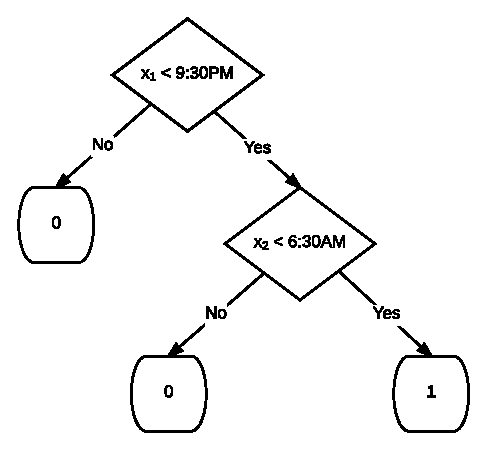
\includegraphics[width=2in]{simple_health}
\end{figure}
\end{minipage}
	
\end{frame}

\begin{frame}\frametitle{Are Models \textit{Really} Deterministic?}

This is an ancient question... it touches on the free will vs. determinism debate.  \pause We will punt on the philosophy and ask: is our model deterministic? \pause NO. \\~\\

Thus, this model is \emph{wrong}. Why?  \pause We can find at least one person who does not have a matching response when inputs are evaluated in $f$. Seems obvious but...

\end{frame}

\begin{frame}\frametitle{Smoking and Lung Cancer}

\small
Consider the model with the binary input 

\begin{itemize}
\item[$y$:] contract lung cancer at some point (1) or not (0)
\item[$x_1$:] smoke 10 pack years or more at some point in a lifetime (1) or not (0) and the response 
\end{itemize} \pause 

Do you think the model should look like the below?\vspace{-0.2cm}

\begin{figure}
\centering
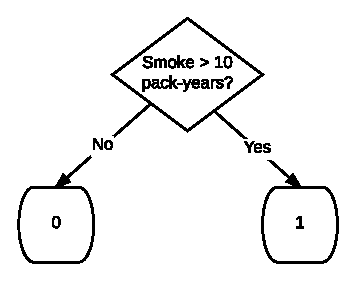
\includegraphics[width=1.4in]{smoking}
\end{figure}
 \pause 


\vspace{-0.2cm}
No... in fact \qu{only} 16\% of smokers get lung cancer compared to about 0.4\% of non-smokers. Thus, the simpel model above is wrong because some responses (that is features of certain individuals) will not \qu{fit} the model. Thus, should we throw out the whole enterprise of modeling?


%http://colinchamp.com/diet-studies-and-cancer/
\end{frame}

\begin{frame}\frametitle{Statistical Models}

Mathematical models such as

\beqn
y = f(x_1, x_2, \ldots)
\eeqn

can become forgiving to \emph{errors} in $f$ by allowing for $y$ to be modeled non-deterministically as a random variable (r.v.), uppercase $Y$. For our case of binary classification, this r.v. is the Bernoulli:

\beqn
Y \sim \bernoulli{f(x_1, x_2, \ldots)} := \begin{cases} 
1 ~~\text{with probability~} f(x_1, x_2, \ldots) \\
0 ~~\text{otherwise}
\end{cases} 
\eeqn

Since the response is now a r.v., we call this a \emph{statistical model}.
	
\end{frame}

\begin{frame}\frametitle{A Statistical Model}

A more conceivable model $f$ is:

\begin{figure}
\centering
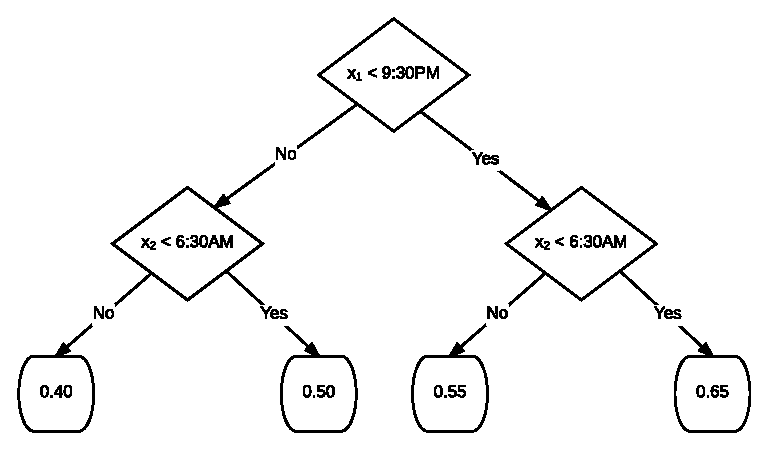
\includegraphics[width=3.2in]{stat_class_model_health}
\end{figure} \pause 

Are there still reasons for $x_1$ and $x_2$ to be rigid binary values e.g. 1 if $x_2 <$ 6:30AM? No... but we haven't spoke about model fits nor parameters.... wait...

\end{frame}

\begin{frame}\frametitle{Is Health Dichotomous?}
\small

So, we should really update the text of the aphorism to reflect the introduction of the random variable response. It should read:

\begin{quotation}
Early to bed and early to rise makes a man \pause  \emph{more likely to be} healthy.
\end{quotation}

However this seems to still suggest someone is either healthy or not healthy. Didn't the author of the aphorism, to be more accurate, say... 

\begin{quotation}
Early to bed and early to rise makes a man \pause  \emph{healthier}.
\end{quotation}

which is deterministic (and we will fix it soon):

\beqn
y = f(x_1, x_2)
\eeqn 

we need some way to measure a quantity of healthiness on a continuous scale.  \pause Open problem. How can you shrink-wrap health into a single number?

\end{frame}

\begin{frame}\frametitle{QOL: a Response Metric?}

\footnotesize
One such scale is found in \href{http://europepmc.org/abstract/med/6460487}{Flanagan (1978)} invented the precursor to the modern \qu{Quality of Life Scale} (QOLS) metric based on assessing 7-point Likert scales. It takes 5 minutes and scores range from 16--112. Here are the categories:

\vspace{-0.2cm}
\begin{figure}
\centering
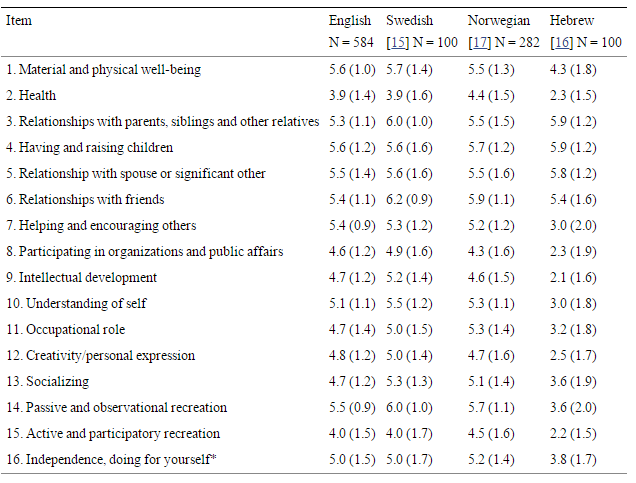
\includegraphics[width=3.2in]{qol_table.png}
\end{figure}

\end{frame}

\begin{frame}\frametitle{Making Up Metrics}

Yes, metrics are essentially \qu{made up}. Good ones are engineered to carefully capture the information sought. Examples:

\begin{itemize}
\item \href{https://www.cato.org/human-freedom-index}{The Human Freedom Index} \pause 
\item \href{https://en.wikipedia.org/wiki/Democracy-Dictatorship_Index}{Democracy-Dictatorship Index} \pause 
\item S\&P 500 \pause 
\item Visual Acuity 20/20, 20/40, etc \pause 
\end{itemize}

It is most important for these metrics to be monotonic (i.e. higher always means better or worse).  \pause 

We also would appreciate these metrics being approximately linear. So an increase of 1 \qu{point} on the scale means the same increase/decrease in quality. But that is usually too much to ask.


	
\end{frame}

\begin{frame}\frametitle{Back to Modeling}

We now are considering health as a continuous number (the data type is called \qu{continuous}) but the model is still deterministic. How to we reengineer the aphorism to allow for stochasticity (randomness)?

\begin{quotation}
Early to bed and early to rise makes a man  \pause \emph{healthier on average}.
\end{quotation}
	
We can then build a statistical model:

\beqn
Y \sim g\parens{f(x_1, x_2), \sigsq, \ldots}
\eeqn

where $f(x_1, x_2)$ now represents the mean health for these inputs, $\sigsq$ is now variance around that mean,  \pause and the ellipses is a technicality dealing with higher moments such as skew, etc that we will ignore for the purposes of this class. Thus, health scores are realized randomly but the mean health scores are deterministic.

\end{frame}

\begin{frame}\frametitle{Regression Models}

\small
When the response is continuous, the statistical model is called a \textit{regression model}. What does regression mean?  \pause Loosely, when you hear regression, you know you're modeling some continuous response (e.g. price, blood pressure, lens power). The typical way these models are written are:

\beqn
Y = f(x_1, x_2) + \errorrv
\eeqn

The equals sign makes us feel like we're back in a deterministic model. But we're not; the $\errorrv$ is a r.v. known as the \qu{noise}. (The British call it the \qu{errors} --- why?)  \pause This r.v. necessarily must have no mean, $\expe{\errorrv} = 0$. Can you explain why? \\~\\ \pause 

Where does $\errorrv$ come from?? Philosophical question... one we will return to soon.

\end{frame}

\begin{frame}\frametitle{Conditional Expectation}

The model can be written even another way to belabor this point:

\beqn
Y = \cexpe{Y}{x_1, x_2} + \errorrv
\eeqn

where $\cexpe{Y}{x_1, x_2}$ is called the \qu{conditional expectation function} or the \qu{conditional mean function} and of course,

\beqn
\cexpe{Y}{x_1, x_2} = f(x_1, x_2)
\eeqn

Specifying the model for $f$ is sometimes called \qu{conditional mean modeling}.

How does one think of $\cexpe{Y}{x_1, x_2}$?
	
\end{frame}

\begin{frame}\frametitle{A mock $\cexpe{Y}{x_1, x_2}$ Illustration}

\begin{figure}
\centering
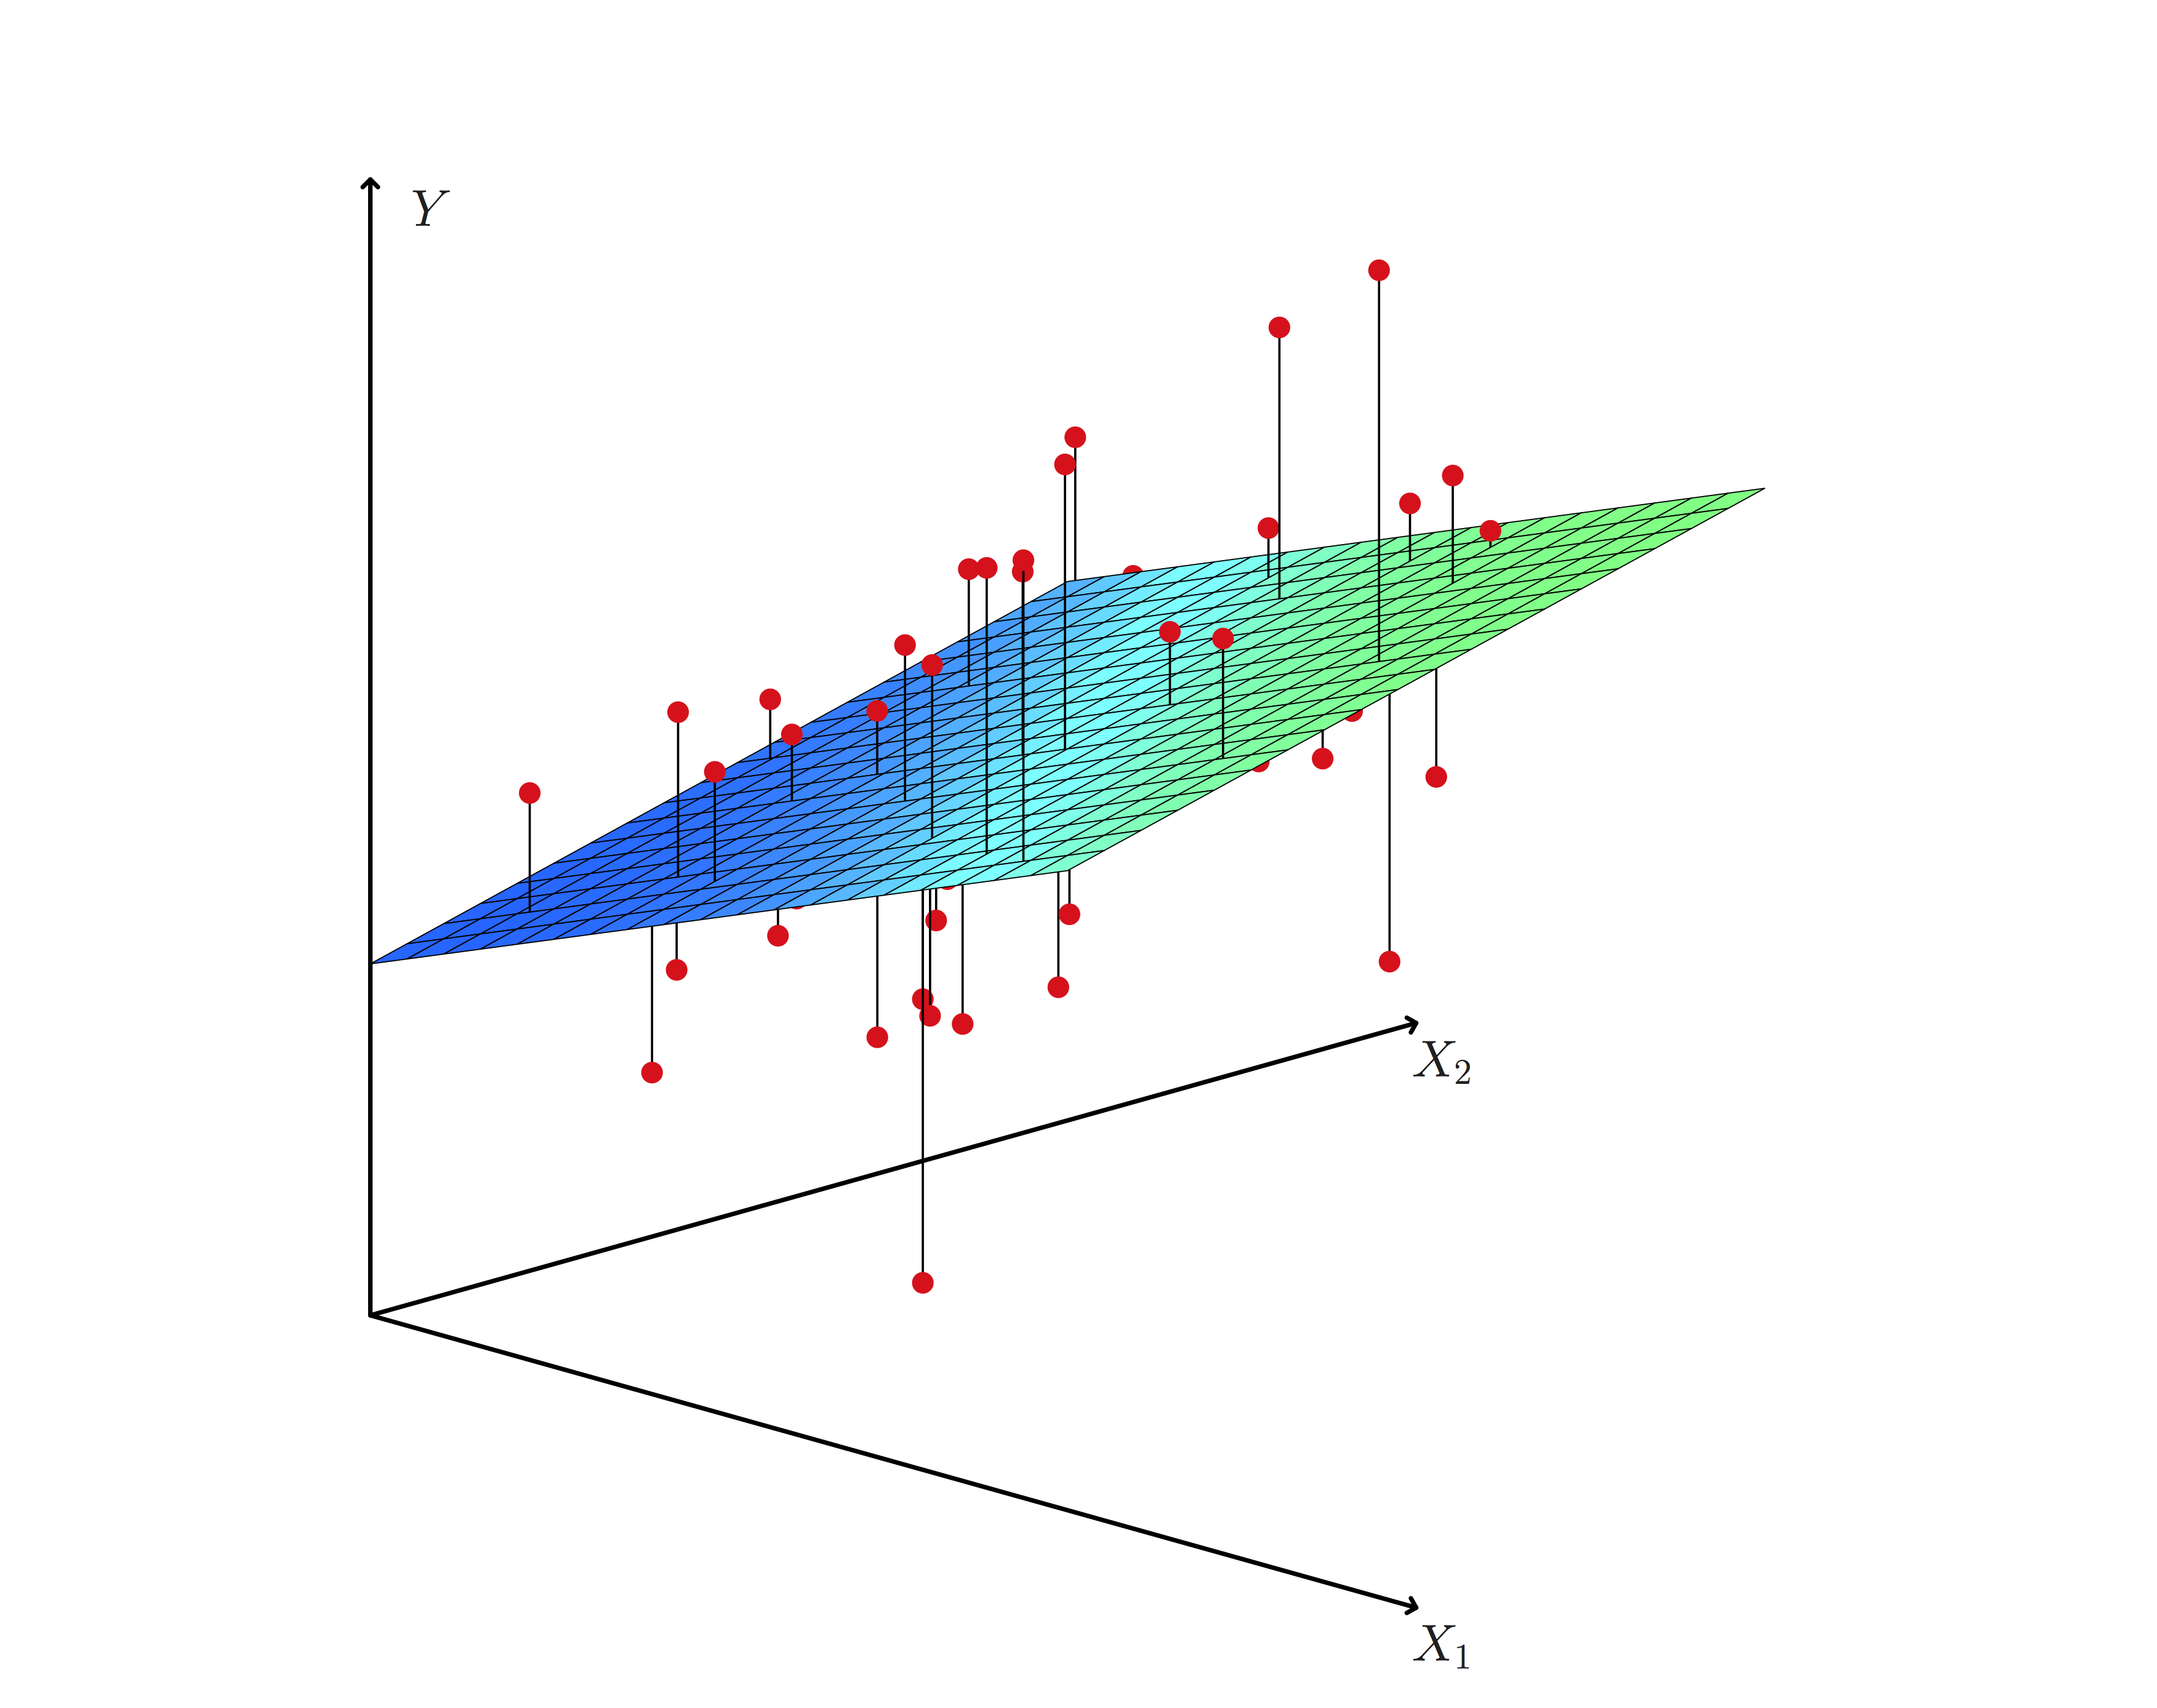
\includegraphics[width=3.45in]{cef.png}
\end{figure}
	
\end{frame}

\begin{frame}\frametitle{Generalizing the Inputs}

\begin{quotation}
Early to bed and early to rise makes a man healthier on average.
\end{quotation}

The wording \qu{early to bed} and \qu{early to rise} seem to smack of  \pause binary inputs. Either it's early or it's late... no in-between values.  \pause Again, it's probably not what the original author had in mind.\\~\\ %%%move this above

Let's reengineer the aphorism again to allow for grey area: \pause 

\begin{quotation}
\emph{The earlier} to bed and the \emph{earlier to} rise makes a man healthier on average.
\end{quotation}

\end{frame}

\begin{frame}\frametitle{Bedtime and Waketime Again}

We began with the average bedtime and waketime and recorded it as a datetime.\\~\\ \pause 

We now need to use continuous measures for $x_1$ and $x_2$. How can we do this? Should we use 9:42PM, 10:14PM, etc. as before? What is later 11:55PM or 1:02AM?\\~\\ \pause 

We should not use timestamps as they fail the monotonicity property that we desire to capture \qu{lateness}.\\~\\ \pause 

What should we do? Maybe just one number defined as the number of hours after an absurd average bedtime like 5PM? Thus, 9PM $\rightarrow x_1 = 4$ and 2AM $\rightarrow x_1 = 9$, etc. Ditto for waketime to avoid the problem of people on average waking up after 12:59PM.
	
\end{frame}

\begin{frame}\frametitle{The Average Is Misleading}

We are using average bedtime and waketime. What's wrong with an average?

\begin{figure}
\centering
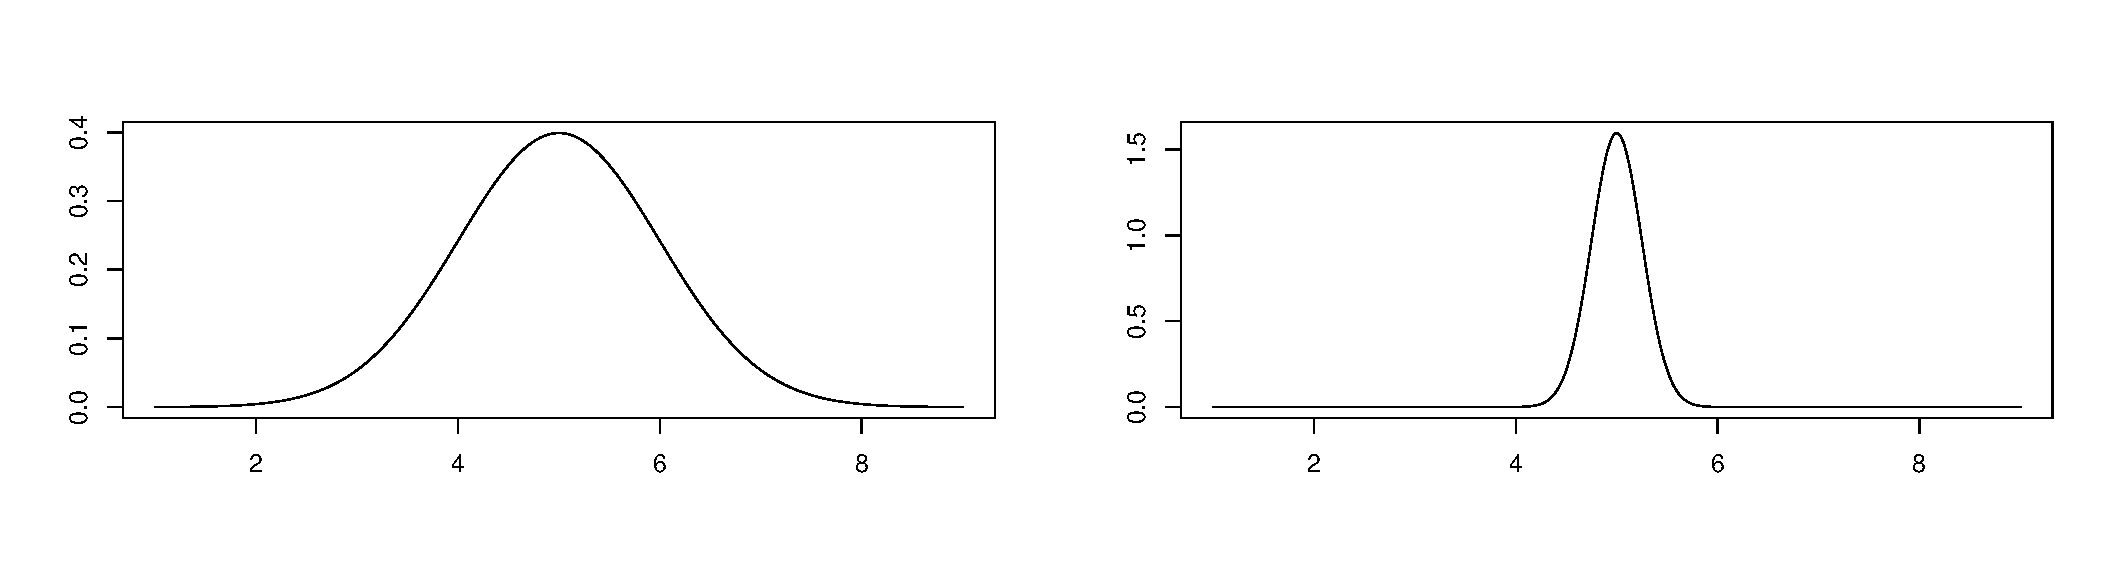
\includegraphics[width=4.5in]{two_dist}
\end{figure}

%par(mfrow = c(1, 2))
%res = 1000
%xs = 5 + seq(-4, 4, length.out = res)
%plot(5 + xs, dnorm(xs, 5, 1), type = 'l', xlab = '', ylab = '')
%plot(5 + xs, dnorm(xs, 5, 0.25), type = 'l', xlab = '', ylab = '')
%
	
These are two bedtime distributions over many, many years. They both have the same average: 10PM. Who do you think is healthier on average?  \pause The person on the right. Why?
\end{frame}

\begin{frame}\frametitle{Designing Better Inputs}

\small
How can we get more \qu{information} out of a person's bedtime and waketime that is relevant to predicting health outcomes? \pause 

We likely don't know which piece of the distribution will be helpful, so let's just add all the information. Let's bin by maybe 20min and record the probabilities over many years of being in that bin. For instance, 5 year bins for these two people may look like:

%par(mfrow = c(1, 2))
%n = 5 * 365
%x1 = rnorm(n, 5, 1)
%x2 = rnorm(n, 5, 0.25)
%hist(x1, prob = TRUE, xlim = c(1,9), xlab = 'bedtimes', ylab = 'probability density estimate', main = '')
%hist(x2, prob = TRUE, xlim = c(1,9), xlab = 'bedtimes', ylab = 'probability density estimate', main = '')
%	
\vspace{-0.2cm}
\begin{figure}
\centering
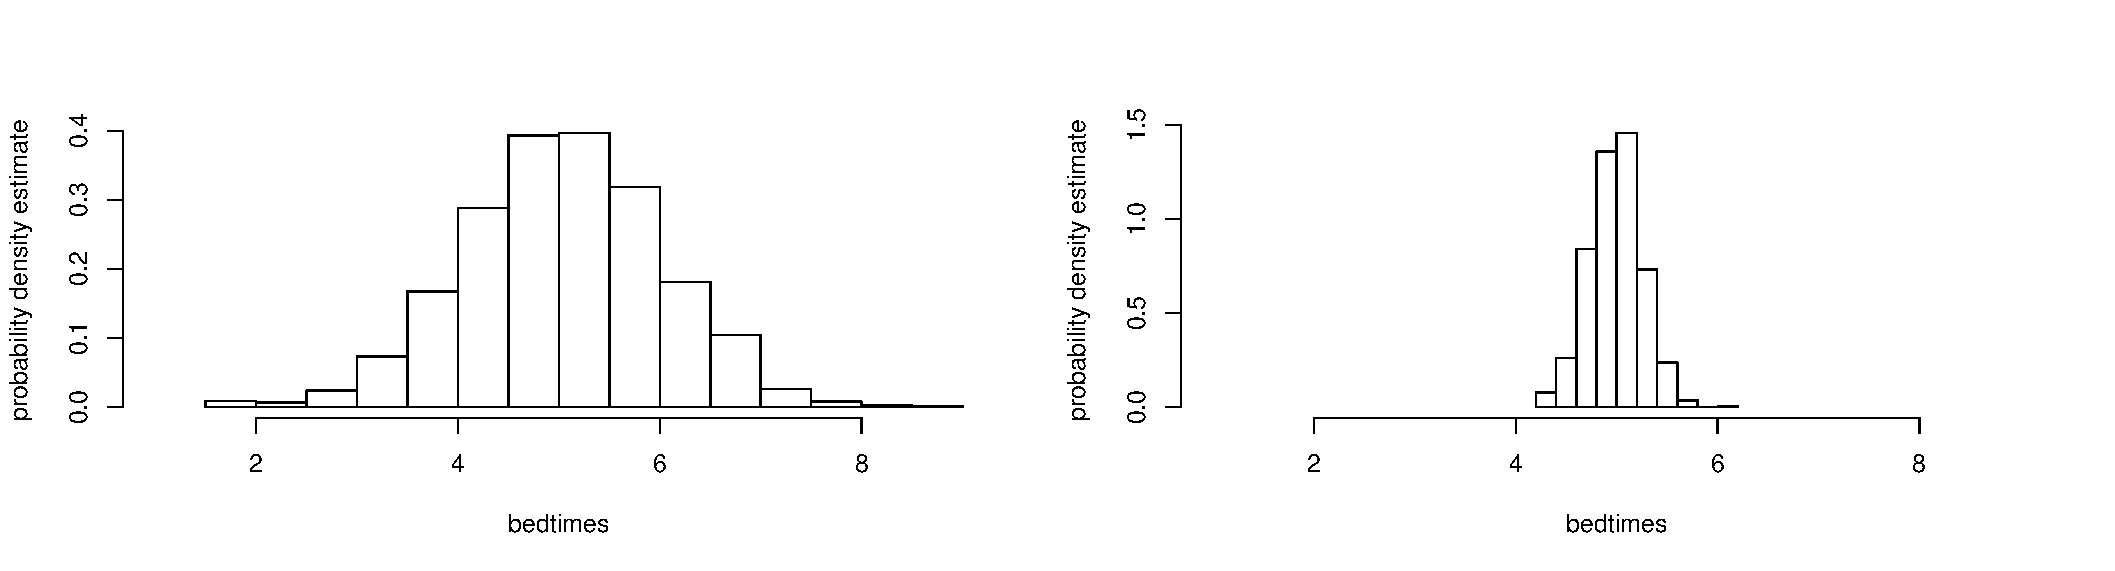
\includegraphics[width=4.5in]{two_hists}
\end{figure}

All bin values can be used as inputs. So in this model, $p > 2$. It could be almost 100. This is called \emph{featurization} --- designing features and we will talk more about it later.

\end{frame}

\begin{frame}\frametitle{Flexible Inputs $p=2 \rightarrow p \approx 100$}

\begin{itemize}
\item Advantage: We can fit more exact rules like if the proportion of times went to bed past 1AM is 10\% ... then health drops considerably and then more so for 2AM \pause 
\item Disadvantage: It makes the model hard to fit and interpret. There are a lot of \qu{degrees of freedom} now (a term you've heard before). A lot more in this later as this is the most important topic in this course.
\end{itemize}

\end{frame}

\begin{frame}\frametitle{Summary}

Models relate inputs to outputs. Inputs and outputs are measurements or assessments on objects / observations.  Here, we consider only one output and name it the response.  \pause All the inputs we then consider to be predictors that explain the response via the model $f$.  \pause 

Data frames have rows that are observations and columns that are predictors (with one column that is a response).  \pause 

Each predictor and the response have a certain data type.  \pause If the data type of the response is categorical (or binary as in two categories), we have a classification model. If the data type of the response is a continuous metric, we have a regression model.
	
\end{frame}

\section{Data Representation \& Parametric Models}

\begin{frame}\frametitle{The Aphorism Revisited}

\small
\begin{quotation}
Early to bed and early to rise makes a man healthy.
\end{quotation}

which may imply binary $x_1$, $x_2$ and $y$ and thus $f$ likely looks like:

\begin{figure}
\centering
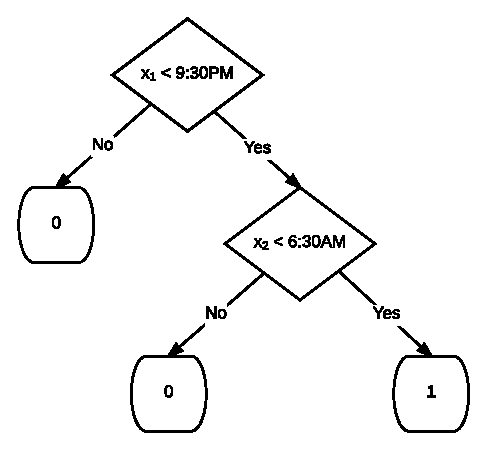
\includegraphics[width=2in]{simple_health}
\end{figure}

New question: where did this model come from??
	
\end{frame}

\begin{frame}\frametitle{History}

\begin{quotation}
As the olde englysshe prouerbe sayth in this wyse. Who soo woll ryse erly shall be holy helthy \& zely.\\
~~- The Book of St. Albans, 1486
\end{quotation}
	
\begin{quotation}
Earely to bed and earely to rise, makes a man healthy, wealthy, and wise. \\
~~- John Clarke's Paroemiologia Anglo-Latina, 1639 (collection of proverbs) \\
~~ -Benjamin Franklin, 1735 (popularized it in American English)
\end{quotation}

We, as a people, built this model and it's been validated over centuries. How did we build it?

\end{frame}

\begin{frame}\frametitle{Humans as Model Builders}

\begin{enumerate}
\item We made it up. Don't laugh... you will see on the homework why this may be subtle. \pause 
\item We used a \qu{data-driven approach}. \\ \pause 

Likely, many individuals independently \textit{observed} people (the unit of observation), assessed both $y$, their healthiness level over their lives and \emph{assessed / measured all features and noted that} their $x_1, x_2$ bedtime and waketime habits were related via a simple pattern relating these inputs to the response. \pause 
\end{enumerate}

\begin{figure}
\centering
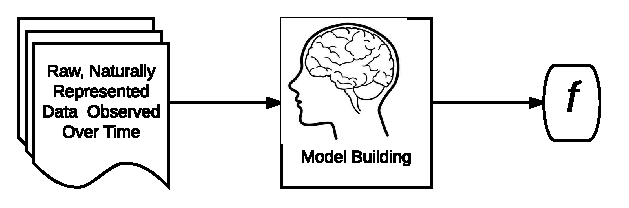
\includegraphics[width=4in]{human_learning}
\end{figure}
	
\end{frame}


\begin{frame}\frametitle{How does this work?}
\small
We notice phenomena around ourselves we wish to explain. For example, a person...

\begin{itemize}
\item ... gets a job at Citadel Capital or not \pause 
\item ... gets a mortgage approved or not \pause 
\item ... runs a mile in $t$ minutes \pause 
\item ... has a degree of healthiness (in our aphorism example)
\end{itemize}

We then pore through the \textit{raw, naturally represented data}. What kind of information is this??\pause 

Everything we notice about the people we observe! Imagine every encounter with the person for years and years (10 minutes here, 5 minutes there), full video clips, audio recordings, smells, touches, tastes, everything. \pause 

How many measurements is that? (What's the dimensionality of the input space?) Immeasurable and cannot be defined. But we know it's HUGE! Note: this is technically called \emph{deep learning}.

\end{frame}


\begin{frame}\frametitle{A Deep Learning Model You've Built}

Is this a cat?

\begin{figure}
\centering
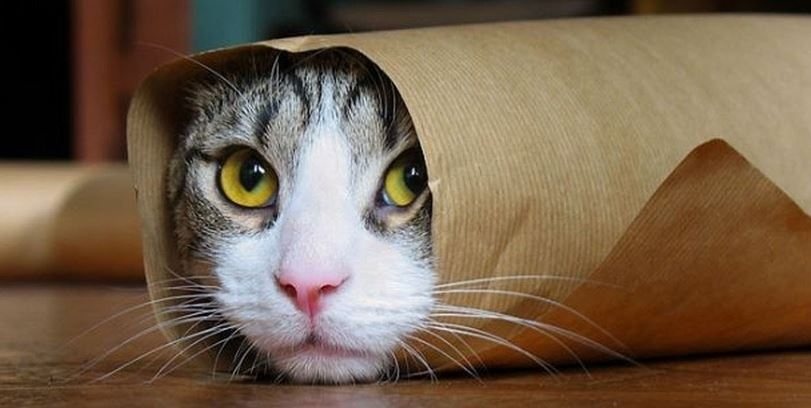
\includegraphics[width=2in]{cat.jpg}
\end{figure}


Response?  \pause Cat or not (0 or 1 numerically). Predictors in the model?  \pause Entire image... raw natural data representation.  \pause The brain shrinks the space down to a small number of predictors. You've already built this model (but only in your head... and you don't even know how it works). 

	
\end{frame}

\begin{frame}\frametitle{Prediction in a Deep-Learned Human Model}


\begin{figure}
\centering
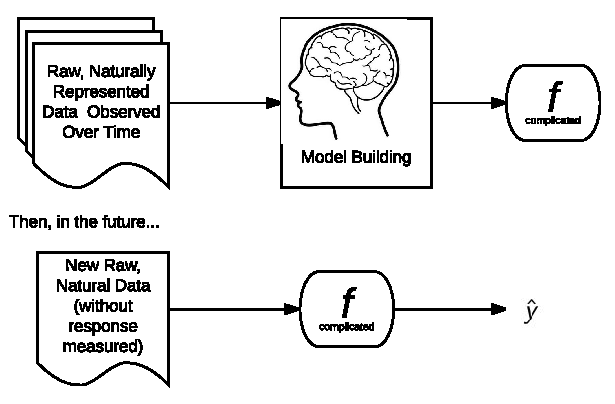
\includegraphics[width=4.3in]{human_learning_weakness}
\end{figure}

\end{frame}

\begin{frame}\frametitle{Weakness in a Deep-Learned Human Model}

\begin{block}{Weaknesses}
\begin{itemize}
\item The model cannot be communicated precisely. \pause 
\item The inputs are too complicated. \pause 
\item The functional form cannot be shared. \pause 
\item And thus no prediction can be made with it (unless it is the same brain that makes the prediction that built the model).
\end{itemize}
\end{block}


	
\end{frame}

\begin{frame}\frametitle{But we Create Simple Models. How?}

\begin{quotation}
Early to bed and early to rise makes a man healthy.
\end{quotation}

\begin{figure}
\centering
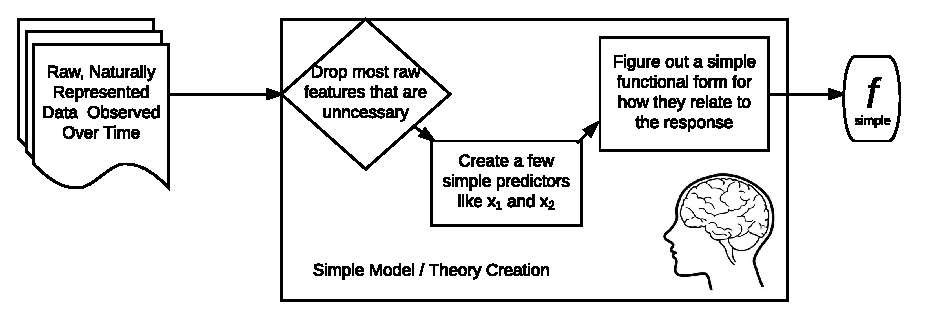
\includegraphics[width=4in]{human_simple_model_learning}
\end{figure}
 \pause 
This is the process by which we put forth the model \qu{early to bed and early to rise makes a man healthy}.

\end{frame}

%The sciences … make models. By a model is meant a … construct which, with the addition of certain verbal interpretations, describes observed phenomena. The justification of such a construct is solely and precisely that it is expected to work. – John von Neumann (1903–1957), 

\begin{frame}\frametitle{Models we are Good and Bad At}
\small

We are ...

\begin{block}{Good at Building Statistical Models when...} \pause 
the number of variables that truly matter is small and there's low noise. %For example: recognizing the face of your friend, understanding speech, etc.
\end{block}
	
\begin{block}{Bad at Building Statistical Models when...} \pause 
inputs are already derivative features of the raw data representation, are numeric and there a lot of them ($p$ large), and noise is large ($\var{\errorrv} >> 0$). %For example, everything we will likely do for the rest of the semester.
\end{block}


\end{frame}

\begin{frame}\frametitle{We are Frequently Bad...}

Famous finding: Paul Meehl in 1954 found when comparing predictions from a panel of clinicians with PhD's and predictions with a linear model (a simple statistical model),  \pause he found the linear model beat the PhD's.


\begin{quotation}\footnotesize
When one is dealing with human lives and life opportunities, it is immoral to adopt a mode of decision-making which has been demonstrated repeatedly to be either inferior in success rate...
\end{quotation} \pause 

The clinicians make a diagnosis on the basis of a quick meeting and a whole bunch of numeric variables: age, serum glucose, blood pressure, symptom measurements... difficult models for us to build.

\end{frame}


\begin{frame}\frametitle{Can we Use Artificial Intelligence (AI)?}

Can we use computers to build models, especially the models we're bad at?  \pause 

\begin{figure}
\centering
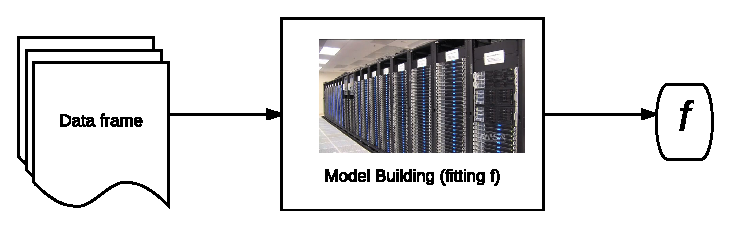
\includegraphics[width=4in]{machine_learning}
\end{figure}
	
Luckily, yes. And this is a main advantage of artificial intelligence.

\end{frame}

\begin{frame}\frametitle{Types of AI?}

\begin{figure}
\centering
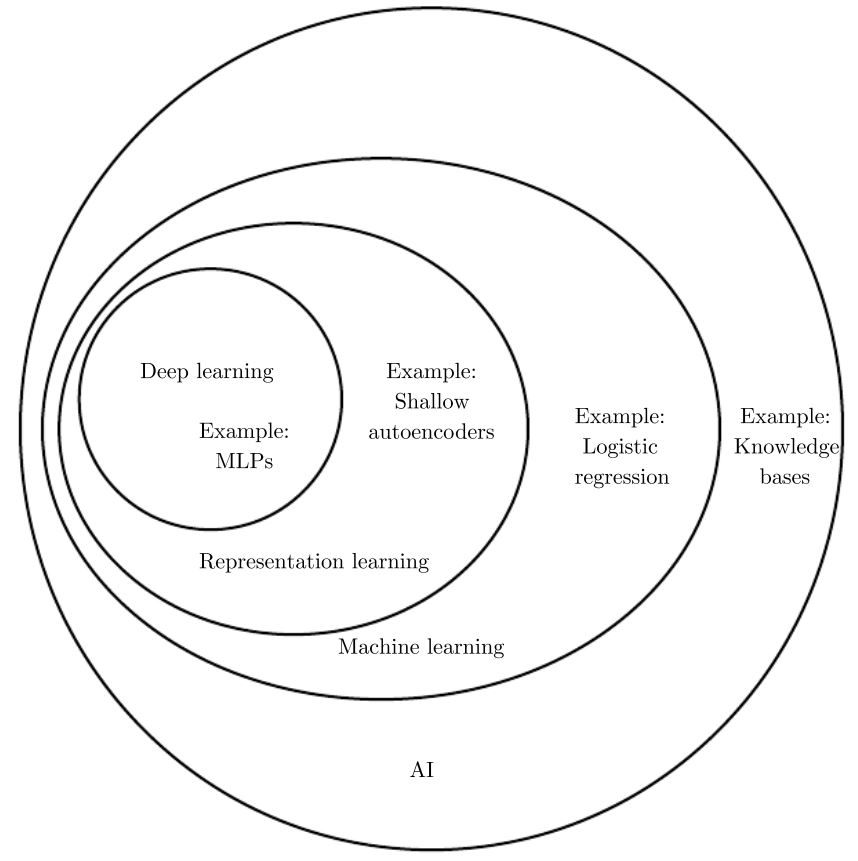
\includegraphics[width=2.5in]{fig14.jpg}
\end{figure}

(Fig 1.4 in Goodfellow et al., 2017)

\end{frame}

\begin{frame}\frametitle{What Does Input to AI Look Like?}

Let's return to our model:\\~\\

\begin{quotation}
Early to bed and early to rise makes a man healthy.
\end{quotation}

We observe every encounter with the person for years and years (10 minutes here, 5 minutes there), full video clips, audio recordings, smells, touches, tastes, everything.\\~\\ \pause 

Can we enter all this into a computer? No, not now, possibly not ever. Also, willl be using statistical modeling so it needs well-defined measurements. So we need to \qu{featurize} and then \qu{collect data}.

	
\end{frame}

\begin{frame}\frametitle{What is Featurization \& Data Collection?}

\begin{figure}
\centering
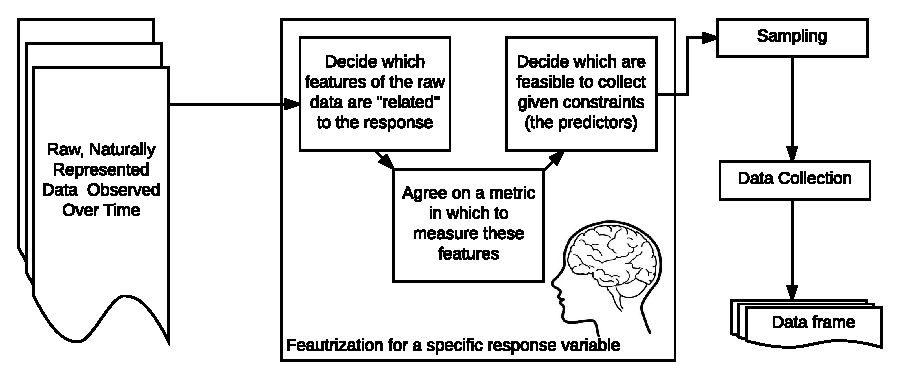
\includegraphics[width=4.5in]{featurization}
\end{figure}

What is featurization?  \pause Deciding predictors. What is data collection?  \pause (a) sampling units then  \pause (b) measuring the numeric values of the predictors  \pause (note: some measurements may be missing).

\end{frame}

\begin{frame}\frametitle{What is Good Machine Learning?}
\begin{figure}
\centering
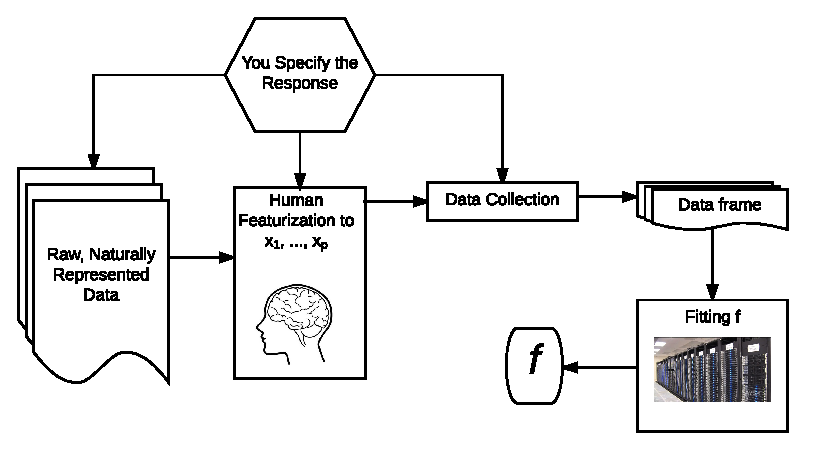
\includegraphics[width=4.5in]{good_machine_learning}
\end{figure}

	
\end{frame}

\begin{frame}\frametitle{What is Day-Day Machine Learning?}
\begin{figure}
\centering
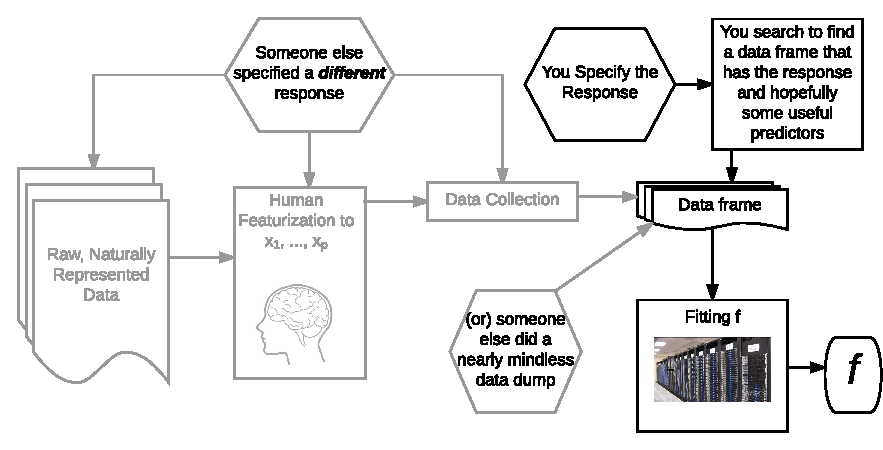
\includegraphics[width=4.5in]{bad_machine_learning}
\end{figure}

This is \emph{bad}... but it's what we generally do all day...
	
\end{frame}

\begin{frame}\frametitle{Baseball Data Questions}

\begin{itemize}
\item Response?
\item Predictors?
\item $n = $? $p = $?
\item How was this data frame likely collected?
\item Do you think by studying this dataset you can predict salaries?
\end{itemize}

	
\end{frame}


\begin{frame}\frametitle{Aside: what is Deep Learning?}
\begin{figure}
\centering
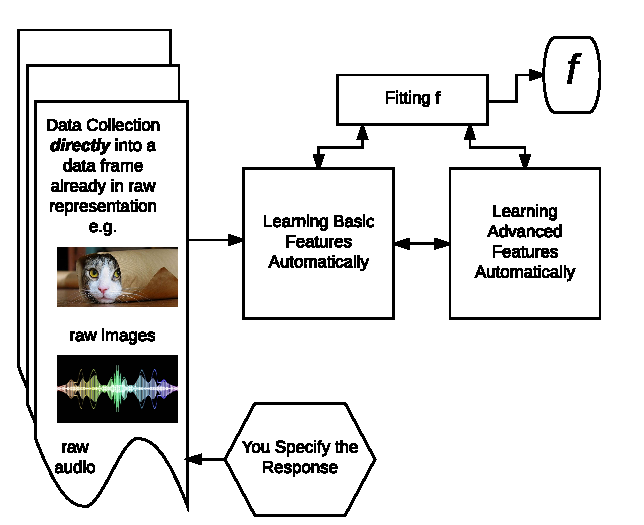
\includegraphics[width=2.9in]{deep_learning}
\end{figure}

Learning complex features automatically (the cutting edge). Software running self-driving cars use this.
%%http://selfdrivingcars.mit.edu/
\end{frame}


\begin{frame}\frametitle{What are we really bad at?}

\begin{figure}
\centering
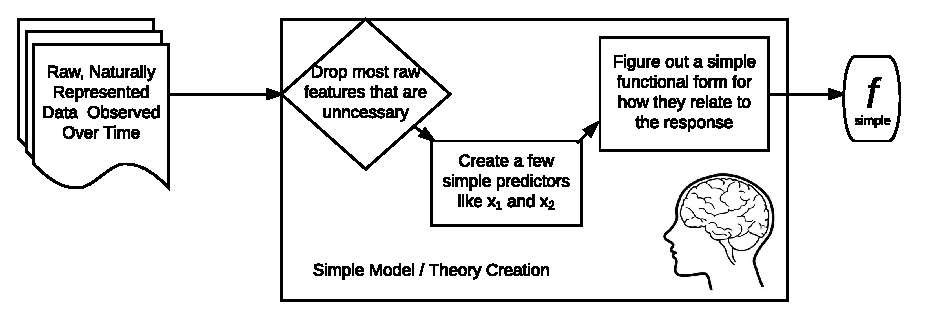
\includegraphics[width=4in]{human_simple_model_learning}
\end{figure}

Figuring out those functional forms... and the computer excels at it.

\end{frame}



\begin{frame}\frametitle{The Fundamental Statistical Problem}


\small
We know our response variable, we've picked features, made measurements and now have an $n \times (p + 1)$ data frame. We know the response looks like 

\beqn
Y = f(x_1, x_2, \ldots, x_p) + \errorrv
\eeqn

where $f$ represents the conditional mean $\cexpe{Y}{x_1, x_2, \ldots, x_p}$ and the $\errorrv$ r.v. is random noise added atop the conditional mean but we don't know $f$! \\~\\ \pause 

So we have to learn / infer $f$ the best we could from the historical dataset. We denote this fit $\fhat$.  \pause What does this mean in the baseball data?
\end{frame}

\begin{frame}\frametitle{Two Worldviews: (I) Parametric}
\beqn
Y = f(x_1, x_2, \ldots, x_p) + \errorrv
\eeqn

\small
\begin{block}{Philosophy of creating the fit, $\fhat$} \pause 
\begin{itemize}
\item We believe that $f$ has a very \qu{nice} form.  \pause 
\item We value \qu{simplicity} because we wholeheartedly believe in Occam's Razor (simplest theory is the one that should be retained). \pause 
\item We love the simple mathematical models such as $V=IR$ and $F = G\frac{m_1 m_2}{d^2}$ and always try to live up to their elegance. \pause 
\item We care very much about knowing how $f$ works inside i.e. how each of the $x_j$ predictors are affect the conditional mean. Knowing how this system works is our top priority. \pause 
\item Absolute prediction accuracy is not our \#1 focus. $f \not \approx \fhat$
\end{itemize}
\end{block}

\end{frame}

\begin{frame}\frametitle{Two Worldviews: (II) Non-Parametric}
\beqn
Y = f(x_1, x_2, \ldots, x_p) + \errorrv
\eeqn
	
\small
\begin{block}{Philosophy of creating the fit, $\fhat$} \pause 
\begin{itemize}
\item We do not make any assumptions about the form of $f$ \qu{nice} or not.  \pause 
\item We have no value for simplicity. We are okay with a world being messy and complex. \pause 
\item We believe simple mathematical models such as $V=IR$ and $F = G\frac{m_1 m_2}{d^2}$ work for idealized situations, but never real-life situations with aribitrarily selected predictors measured in arbitrary ways. \pause 
\item We would like to know how $f$ works, but it's likely very complex, so it's not our top priority. \pause 
\item Absolute prediction accuracy is indeed our \#1 focus. It's the bottom line. We want $f \approx \fhat$ as close as possible.
\end{itemize}
\end{block}
\end{frame}

\begin{frame}\frametitle{Two Worldviews}


The process to find $\fhat$ is known by many names:

\begin{minipage}{0.5\textwidth}
\begin{itemize}
\item parametric modeling
\item model fitting
\item statistical modeling
\item white box modeling
\begin{figure}
\hspace{-1cm}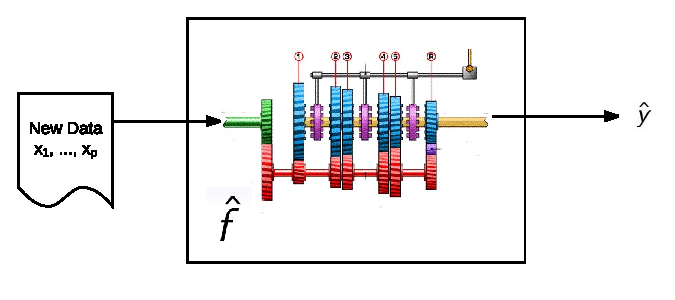
\includegraphics[width=2.0in]{whitebox}
\end{figure}
\end{itemize}
\end{minipage}%
\begin{minipage}{0.5\textwidth}
\begin{itemize}
\item non-parametric modeling
\item function fitting
\item function approximation
\item response surface methodology
\item machine learning
\item black box modeling
\begin{figure}
\centering
\hspace{-0.5cm}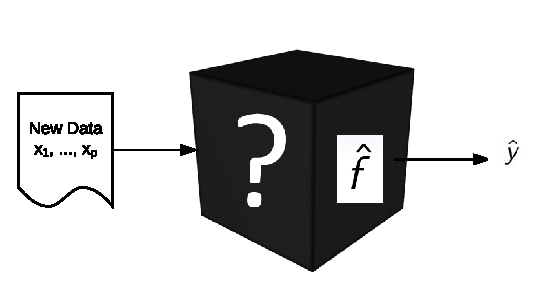
\includegraphics[width=1.8in]{blackbox}
\end{figure}
\end{itemize}
\end{minipage}

\end{frame}

\begin{frame}\frametitle{What is a Parametric Model?}

If we see $f$ is a parametric model, we mean that

\beqn
f(x_1, x_2, \ldots, x_p) \approx s(x_1, x_2, \ldots, x_p; \theta_1, \theta_2, \ldots, \theta_\ell)
\eeqn

i.e. $f$ has a assjumed simple form $s$ that has various knobs that can be adjusted based on the data.  \pause These knobs are called the \emph{unknown parameters}. Here there are $\ell$ of them $\theta_1, \theta_2, \ldots, \theta_\ell$. It is said the model has $\ell$ \qu{degrees of freedom}.  \pause An example of this is the linear model,

\beqn
s(x_1, x_2, \ldots, x_p) = \beta_0 + \beta_1 x_1 + \ldots + \beta_p x_p
\eeqn

with $p$ predictors, there are $p+1$ degrees of freedom (the intercept is also a knob that can be twisted). It is traditional to call the $\theta$'s in the linear model $\beta$'s due to historical reasons.
	
\end{frame}


\section{Fitting the Linear Model}

\begin{frame}\frametitle{What is $\fhat$ in a linear model?}

Then we need to create a fit $\fhat$ that means we need estimates of all the parameters:

\beqn
\fhat(x_1, x_2, \ldots, x_p) = \betahat_0 + \betahat_1 x_1 + \ldots + \betahat_p x_p
\eeqn

then we can use $\fhat$ on new data (where the response is not observed), say $x^*_1, x^*_2, \ldots, x^*_p$ to get a prediction:

\beqn
\yhat = \fhat(x^*_1, x^*_2, \ldots, x^*_p)
\eeqn


Where do we get $\braces{\betahat_0, \betahat_1,  \ldots, \betahat_p}$ from?
	
\end{frame}

\begin{frame}\frametitle{What defines a good fit?}

\small

Consider the simple linear regression (one predictor) i.e. $s(x) = \beta_0 + \beta_1 x$ thus we need to figure out $\betahat_0$ and  $\betahat_1$, constituting the model fitting. Let's say given data, we guess that $\betahat_0 = 7.2$ and $\betahat_1 = -2.8$. Would this be a good fit?

\vspace{-0.5cm}
\begin{figure}
\centering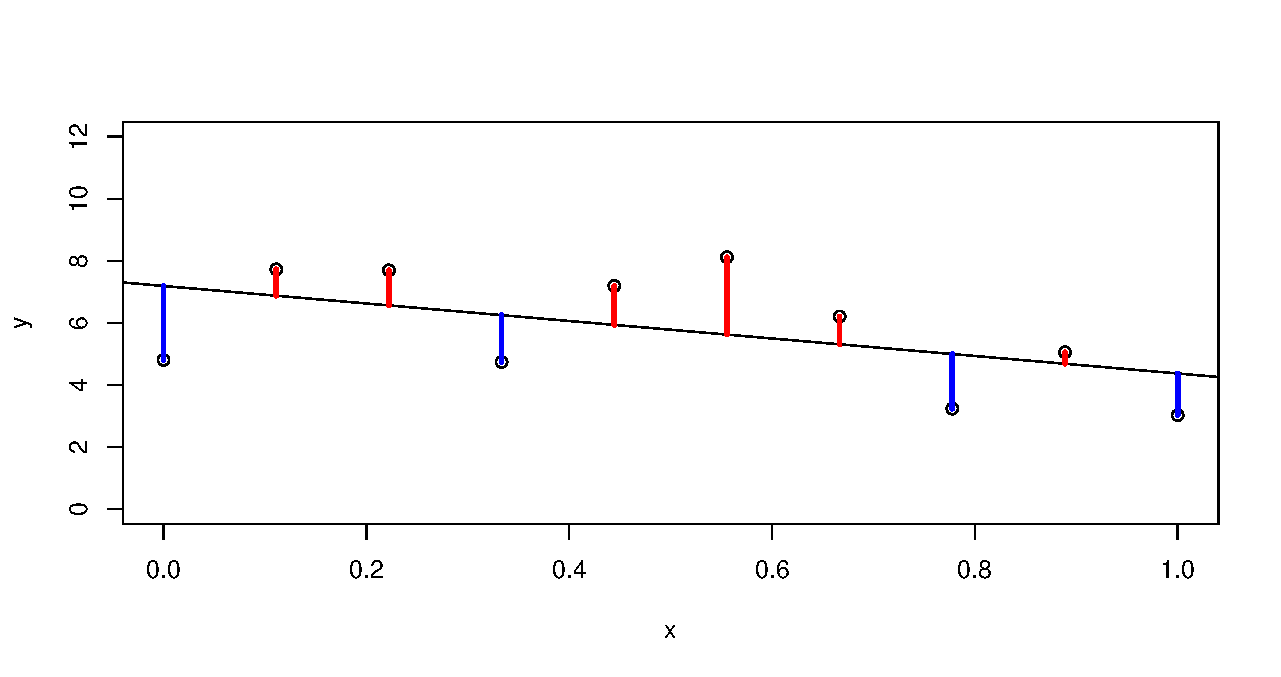
\includegraphics[width=3.0in]{residuals}
\end{figure}

The line is our $\yhat(x)$ i.e. all possible predictions. Seems sometimes we undershot the response (the red) i.e. $y - \yhat > 0$ and sometimes overshot the response (the blue) i.e. $y - \yhat < 0$.

	
\end{frame}

\begin{frame}\frametitle{The Role of the Residuals}

We call $e_i := y_i - \yhat_i$ the $i$th residual. Since we fit all of our historical data there are $n$ residuals $e_1, \ldots, e_n$. Wouldn't it be nice to keep these small? \pause 

\begin{block}{How to create $\fhat$}
\begin{itemize}
\item Minimize $e_1, \ldots, e_n$ while
\item staying true to our assumption $s(x_1, x_2, \ldots, x_p) = \beta_0 + \beta_1 x_1 + \ldots + \beta_p x_p$
\end{itemize}
\end{block}

What does \qu{minimize $e_1, \ldots, e_n$} mean? \pause  We need to define an overall error metric. This is called the \emph{loss function}.
	
\end{frame}


\begin{frame}\frametitle{Loss Functions}

\small
Let $L = L(e_1, \ldots, e_n)$ be a loss function. What's the best we can do?  \pause If we have $e_1 = 0, \ldots, e_n = 0$, then we have no error whatsover. Thus $L \geq 0$. \pause  It is common to sum up the individual losses for each residual. Here are some loss functions below:

\begin{itemize}
\item $L = \abss{e_1} + \abss{e_2} + \ldots + \abss{e_n} = \sum_{i=1}^n \abss{e_i}$ \\ \pause 
This is known as L1 error or absolute error or sum of absolute error \pause 
\item $L = e_1^2 + e_2^2 + \ldots + e_n^2$  \\ \pause 
This is known as L2 error or sum of squared error (SSE) \pause 
\end{itemize}

Linear model fitting and machine learning algorithms mostly use SSE.

\begin{block}{How to create $\fhat$} \pause 
\begin{itemize}
\item Minimize SSE via a  \pause 
\item search over all possible values of $\braces{\betahat_0, \betahat_1,  \ldots, \betahat_p}$
\end{itemize}
\end{block}
 \pause 
Luckily the computer does all of this for you and it just pops out its answer $\betahat_0, \betahat_1,  \ldots, \betahat_p$.
	
\end{frame}

\begin{frame}\frametitle{Is Minimal SSE what you ACTUALLY want?}

Imagine your response is how much IBM stock moves on a percentage basis for one trading day. Consider two scenarios:\\~\\ \pause 

\begin{itemize}
\item If $y = -0.25\%$ and $\yhat = 0.5\%$ then $e = -0.25\% - 0.5\% = -0.75\%$ and the squared loss for your prediction would be 0.00005625.  \pause 
\item If $y = 1.25\%$ and $\yhat = 0.5\%$ then $e = 1.25\% - 0.5\% = 0.75\%$ and the squared loss for your prediction would be 0.00005625. 
\end{itemize}
	
The loss that the \qu{computer sees} for both scenarios is the same. But isn't the first prediction \qu{worse for you} than the second prediction? \\~\\ \pause 

We won't have time to get into custom and asymmetric cost functions. But you need to keep this in mind when you consider the predictions you make with all of the $\fhat$'s we discuss in this class.
\end{frame}

\begin{frame}\frametitle{An Interpretable Measure of Fit}

\small
Let $L = L(e_1, \ldots, e_n) = SSE$ be our loss function. Okay, SSE = 654.4567. Did the model fit well?   \pause What are the units of SSE?  \pause The response units squared.  \pause It also grows linearly with $n$. We cannot compare models using SSE.\\~\\

Consider a dataset for income among HS grads that didn't go to college. You have $n=1,000$ historical responses (the incomes). Here they are:

\vspace{-0.25cm}
\begin{figure}
\centering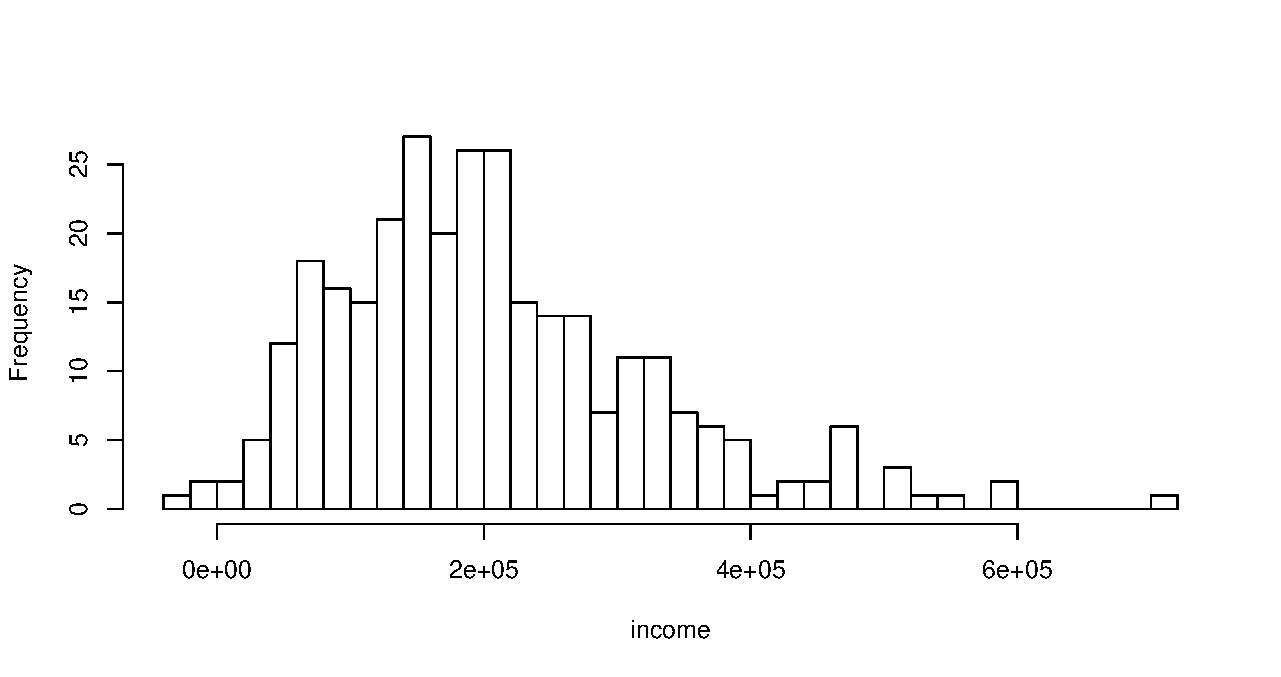
\includegraphics[width=2.7in]{incomes}
\end{figure}
 \pause 
	
\vspace{-0.25cm}
Imagine there was no predictors but you still would like to produce predictions. What would you do?
\end{frame}

\begin{frame}\frametitle{Shoot Blind}

The best guess (i.e. the one with minimal SSE) is the average $\yhat = \ybar$ for any new observation. Using this prediction model, albeit very basic, the SSE is 115512239042 (usually called SST). \pause 

Now imagine you had a predictor... let's say some measure of work ethic or intelligence, call it $x$. Here's a plot:

\vspace{-0.25cm}
\begin{figure}
\centering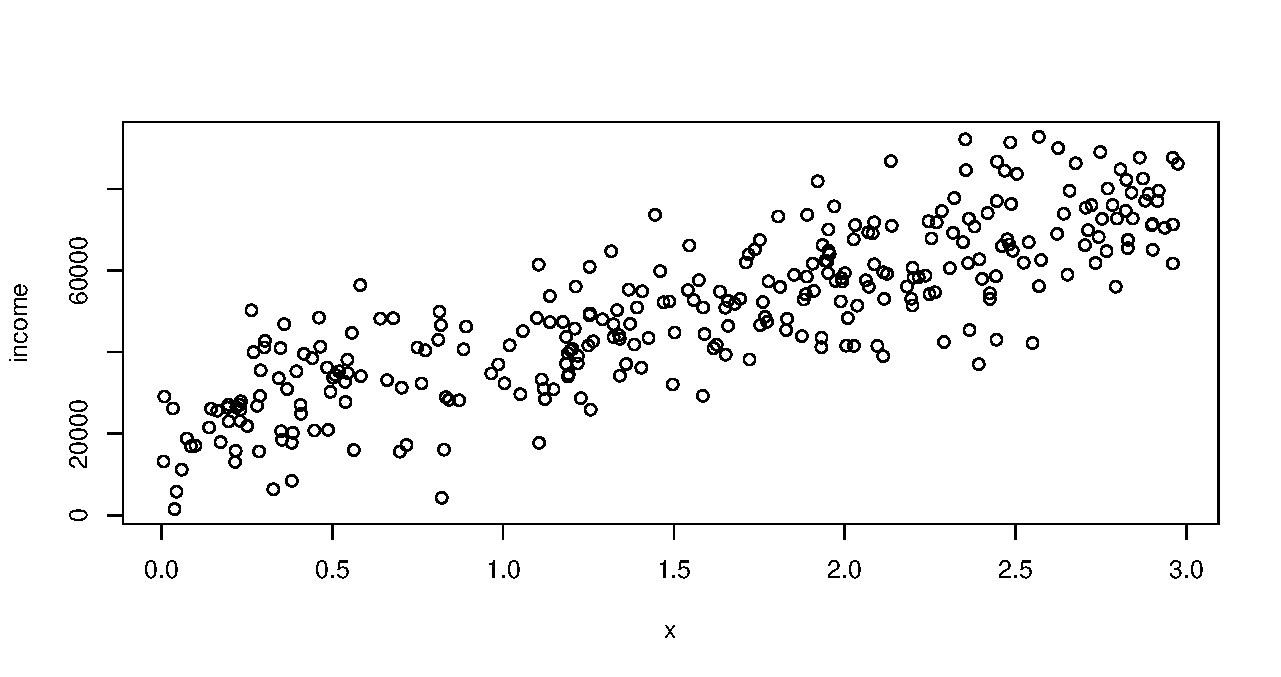
\includegraphics[width=2.7in]{income_by_x}
\end{figure}
	
(see in R)


\end{frame}

\begin{frame}\frametitle{Shoot Less Blind}

\small
Now, the \qu{new} SSE is 34198974577. \pause  This is a reduction in SSE by 81313264465 or as a percentage basis 81313264465 / 115512239042 = 70.39\%. Seen this before? \pause 

\beqn
R^2 := \frac{SSE_0 - SSE}{SSE_0}
\eeqn

Why is this called \qu{percentage of variance explained}? \pause 

\beqn
R^2 &:=& \frac{SSE_0 - SSE}{SSE_0} \times \frac{n-1}{n-1} = \frac{\oneover{n-1}SSE_0 - \oneover{n-1}SSE}{\oneover{n-1}SSE_0} \\
&=& \frac{\oneover{n-1}\sumionen{\squared{y_i - \ybar}} - \oneover{n-1}\sumionen{\squared{y_i - \yhat_i}}}{\oneover{n-1}\sumionen{\squared{y_i - \ybar}}} \\
&=& \frac{s^2_y - s^2_e}{s^2_y} \approx \frac{\var{Y} - \var{E}}{\var{Y}} 
\eeqn

where $\var{Y}$ is what was inexplicable before and $\var{E}$ is what is inexplicable after. $R^2$ is really an \textit{estimate} of the pctg var. explained.
\end{frame}

\begin{frame}\frametitle{Limitations of $R^2$}

$R^2$ is the great equalizer among all models and all responses. They are immediately comparable. But $R^2$ doesn't mean much for my specific problem. \pause  I'm now predicting income, $\yhat = \$70,000$ and $R^2 = 70\%$. How does knowing $R^2 = 70\%$ (i.e. the model fit is pretty good) tell me how good my $\yhat$ is?  \pause How big is $e$ in $y = \yhat + e$ where $y$ is the true response for this prediciton. It doesn't...\\~\\

How about the following metric? \pause 

\beqn
s_e = \sqrt{s^2_e} = \sqrt{\oneover{n-1} SSE}= \sqrt{\oneover{n-1}\sumionen{\squared{y_i - \yhat_i}}}
\eeqn

This is our best guess of the standard error of our estimate $e$, our residual (AKA \qu{RMSE}). What is a standard error?

\end{frame}

\begin{frame}\frametitle{Recall the Empirical Rule}

If $X \sim \normnot{\mu}{\sigsq}$, then 

\begin{itemize}
\item $\mu \pm 1 \sigma$ contains 68\% of the realization values
\item $\mu \pm 2 \sigma$ contains 95\% of the realization values
\item $\mu \pm 3 \sigma$ contains 99.7\% of the realization values
\end{itemize} \pause 

Thus for a realization $x$,

\begin{itemize}
\item $x \pm 1 \sigma$ contains $\mu$ 68\% of the time
\item $x \pm 2 \sigma$ contains $\mu$ 95\% of the time
\item $x \pm 3 \sigma$ contains $\mu$ 99.7\% of the time
\end{itemize}

\end{frame}

\begin{frame}\frametitle{Stretch the Empirical Rule}

If $\sigma$ is unknown then,

\begin{itemize}
\item $x \pm 1 s$ contains $\mu$ about 68\% of the time
\item $x \pm 2 s$ contains $\mu$ about 95\% of the time
\item $x \pm 3 s$ contains $\mu$ about 99.7\% of the time
\end{itemize} \pause 

and if the distribution of $X$ is non-normal but not too funky,

\begin{itemize}
\item $x \pm 1 s$ contains $\mu$ about about 68\% of the time
\item $x \pm 2 s$ contains $\mu$ about about 95\% of the time
\item $x \pm 3 s$ contains $\mu$ about about 99.7\% of the time
\end{itemize}

\end{frame}

\begin{frame}\frametitle{Why is RMSE useful?}

\small
In our case, the r.v. is $Y~|~X_1, \ldots, X_p$ which is centered at $\mu = \cexpe{Y}{x_1, \ldots, x_p}$ and generally speaking, non-normal. $\yhat \approx \mu$ and $s_e \approx \se{Y~|~X}$. Thus, \pause 

\begin{itemize}
\item $\yhat \pm 1 s_e$ contains 68\% of the response values for a specific $x_1, \ldots, x_p$
\item $\yhat \pm 2 s_e$ contains 95\% of the response values for a specific $x_1, \ldots, x_p$
\item $\yhat \pm 3 s_e$ contains 99.7\% of the response values for a specific $x_1, \ldots, x_p$
\end{itemize}

Thus RMSE gives you an approximate means of assessing how variable the real response $y$ could be give your predicted response $\yhat$ .


\end{frame}


\begin{frame}\frametitle{All Three are Equivalent}

Minimizing SSE, maximizing $R^2$ and minimizing $s_e$ all give equivalent fits.
\beqn
SSE, && \\
R^2 &:=& \frac{SSE_0 - SSE}{SSE_0} ~~\text{and} \\
s_e &=& \sqrt{s^2_e} = \sqrt{\oneover{n-1} SSE}= \sqrt{\oneover{n-1}\sumionen{\squared{y_i - \yhat_i}}}
\eeqn


\end{frame}



\begin{frame}\frametitle{Inference}

We haven't spoken about $t$ tests. Why is that? \\~\\ \pause 

In order to have inference, we need to make explicit random variable model assumptions

\beqn
Y \sim g( \beta_0 + \beta_1 x_1 + \ldots + \beta_p x_p, \sigsq, \ldots)
\eeqn

must be assumed to be something like

\beqn
Y \sim \normnot{\beta_0 + \beta_1 x_1 + \ldots + \beta_p x_p}{\sigsq}
\eeqn
	
(we will explore next time) \\~\\

	
\end{frame}


\begin{frame}\frametitle{$R^2$ vs. $F$ test}

In this case $R^2$ will be related to $F$, the omnibus test statistic for whether the model has any signal whatsoever.

\beqn
R^2 = \frac{SSE_0 - SSE}{SSE_0} = \ldots = 1 - \inverse{1 + F \frac{p-1}{n-p}}
\eeqn

\beqn
F &=& \frac{\frac{SSE_0 - SSE}{p - 1}}{\frac{SSE}{n-p}} = \frac{SSE_0 - SSE}{SSE} \frac{n-p}{p-1} = \ldots \\
&=& \underbrace{\frac{R^2}{1-R^2}}_{
%
\substack{
\text{ratio of variance} \\ 
\text{explained to} \\ 
\text{unexplained}
}} 
%
\underbrace{\frac{n-p}{p-1}}_{\substack{
\text{penalty for} \\ 
\text{too many features}
}}
\eeqn


\end{frame}

\end{document}
%\section{Correlation  $\not \Rightarrow$  Causation}
%
%\begin{frame}\frametitle{A \qu{Causal} Model}
%
%\begin{quotation}
%The earlier to bed and the earlier to rise \emph{makes} a man healthier on average.
%\end{quotation}
%
%What does the language suggest by using the verb \qu{to make}? It suggests that the \qu{earlier to bed and the earlier to rise} \textit{causes} \qu{a man [to be] healthier on average}.
%	
%\end{frame}



\begin{frame}\frametitle{}

	
\end{frame}

\begin{frame}\frametitle{}

	
\end{frame}


\begin{frame}\frametitle{}

	
\end{frame}

\begin{frame}\frametitle{}

	
\end{frame}


\begin{frame}\frametitle{}

	
\end{frame}

\begin{frame}\frametitle{}

	
\end{frame}


\begin{frame}\frametitle{}

	
\end{frame}

\begin{frame}\frametitle{}

	
\end{frame}


\begin{frame}\frametitle{}

	
\end{frame}

\begin{frame}\frametitle{}

	
\end{frame}


\begin{frame}\frametitle{}

	
\end{frame}

\begin{frame}\frametitle{}

	
\end{frame}


\begin{frame}\frametitle{}

	
\end{frame}

\begin{frame}\frametitle{}

	
\end{frame}


\begin{frame}\frametitle{}

	
\end{frame}

\begin{frame}\frametitle{}

	
\end{frame}


\begin{frame}\frametitle{}

	
\end{frame}

\begin{frame}\frametitle{}

	
\end{frame}


\begin{frame}\frametitle{}

	
\end{frame}

\begin{frame}\frametitle{}

	
\end{frame}


\begin{frame}\frametitle{}

	
\end{frame}

\begin{frame}\frametitle{}

	
\end{frame}


\begin{frame}\frametitle{}

	
\end{frame}

\begin{frame}\frametitle{}

	
\end{frame}


\begin{frame}\frametitle{}

	
\end{frame}

\begin{frame}\frametitle{}

	
\end{frame}

\end{document}


